\documentclass[11pt, a4paper]{article}
\usepackage[nochapters]{classicthesis}                              % template
\usepackage[margin=42mm]{geometry}                                  % margins
\usepackage[utf8]{inputenc}                                         % allow utf-8 input
\usepackage[T1]{fontenc}                                            % use 8-bit T1 fonts
\usepackage{graphicx}                                               % images
\usepackage{url}                                                    % URL typesetting
\usepackage{booktabs}                                               % good-looking tables
\usepackage{multirow}                                               % for tables
\usepackage{amsfonts}                                               % blackboard math symbols
\usepackage{amsmath}                                                % math ops
\usepackage{nicefrac}                                               % compact 1/2, etc.
\usepackage{microtype}                                              % microtypography

\definecolor{darkblue}{rgb}{0, 0, 0.5}                              % define link color
\hypersetup{colorlinks=true,citecolor=darkblue,                     % set link color
            linkcolor=darkblue, urlcolor=darkblue}

% Your packages here
% \usepackage{...}                                                  % some info, maybe

% !!! PLEASE CHANGE THESE VARIABLES TO MATCH YOUR INFORMATION !!!

\def\thesistitle{Measuring Domain-Specific Sentiment to Predict Stock Prices}                      % title
\def\subtitle{The WallStreetBets 'Meme-Stock' Saga}             % subtitle
    % ^if there is no subtitle, replace by \def\subtitle{}  
\def\yourname{Stefan Winter}                                                                       % ^first and last name
\def\yourprogramme{Data Science \& Society}                         % OR (remove this)
% \def\yourprogramme{Cognitive Science \& Artificial Intelligence}    % uncomment this
\def\yourstudentnumber{2067606}                                      % ANR (or u-number)
\def\finalmonth{January}
\def\finalyear{2022}
\def\supervisor{Dr. Peter Hendrix}
\def\committee{Dr. Raquel Garrido Alhama}
\def\acknowledgments{I want to thank Dr. Peter Hendrix for his invaluable guidance during this thesis.}

% METADATA

\hypersetup{pdfauthor   = \yourname,
            pdftitle    = \thesistitle\ \subtitle,
            pdfsubject  = \yourprogramme\ Master Thesis
}

% CHOOSE EITHER OF -----------------------------------------
% IEEE STYLE:

% \usepackage[square,numbers]{natbib}                               % bracket-style refs
% \usepackage{natbib}                                               % OR: parenthesized refs
% \bibliographystyle{IEEEtranN}

% OR -------------------

\usepackage[natbibapa]{apacite}                                     % only parentheses
\bibliographystyle{apacite}                                         % 'cause APA

% !!! ------------------------------------------------------ !!!

\begin{document}

% DON'T TOUCH THIS FILE, THANKS!

\pagenumbering{gobble}
\thispagestyle{empty}

\newgeometry{margin=30mm}
\begin{center}
\hspace{0.75cm}
\includegraphics[scale=0.5]{logo.eps} \\
\vspace{5cm}
\huge\spacedallcaps{\thesistitle} \\ [0.5cm]
\Large\spacedallcaps{\subtitle} \\ [1.2cm]
\normalsize\spacedallcaps{\yourname{}} \\ [1cm]
\normalsize{\spacedlowsmallcaps{Thesis submitted in partial fulfillment}} \\
\normalsize{\spacedlowsmallcaps{of the requirements for the degree of}} \\
\normalsize{\spacedlowsmallcaps{Master of Science in \yourprogramme{}}}\\
\normalsize{\spacedlowsmallcaps{at the School of Humanities and Digital Sciences}} \\
\normalsize{\spacedlowsmallcaps{of Tilburg University}} \\ [1.5cm]
\end{center}
\restoregeometry

\newpage

\begin{tabular}{l}
\noindent \spacedlowsmallcaps{student number} \\ [0.2cm]
\yourstudentnumber \\ [0.5cm]
\spacedlowsmallcaps{Committee} \\ [0.2cm]
\supervisor \\
\committee\\ [0.5cm]
\spacedlowsmallcaps{location} \\ [0.2cm]
Tilburg University    \\                        
School of Humanities and Digital Sciences \\
Department of Cognitive Science \& \\
Artificial Intelligence \\
Tilburg, The Netherlands \\ [0.5cm]
\spacedlowsmallcaps{date} \\ [0.2cm]
\today \\ \\
\spacedlowsmallcaps{Word Count} \\ [0.2cm]
8700 words
\end{tabular}
\vfill
\begin{tabular}{l}
\spacedlowsmallcaps{acknowledgments} \\ [0.2cm]
\noindent \acknowledgments{} \\ \\
\end{tabular}

\newpage

\newpage \pagenumbering{arabic}

\title{\rmfamily\normalfont\spacedallcaps{\thesistitle}\\[0.2cm]
       \rmfamily\small\spacedallcaps{\subtitle}}
\author{\spacedlowsmallcaps{\yourname}}
\date{}

\maketitle  % don't remove this :)

% --- start writing below:

\begin{abstract}
    Until the GameStop short-squeeze in early 2021, the impact of changes in investor-sentiment of the Reddit discussion board \emph{WallStreetBets} on the financial market 
    was vastly underappreciated. 
    Due to the novelty of the WallStreetBets phenomenon, there is also almost no research available on that topic.
    This thesis will explore methodologies on how to measure sentiment of the discussion board and use the sentiment to predict changes of the GameStop stock price.
    One of the challenges when measuring the sentiment of WallStreetBets is the usage of novel 
    domain-specific words and terminologies, which are shown to have a big impact on the results of sentiment analysis models. Hence, this thesis proposes a method 
    to create a labeled dataset that covers the sentiment of text data, including the terminology of a given domain. It will be shown that supervised sentiment analysis machine 
    learning models that use the domain-specific text corpus as input outperform general purpose lexicons, which are currently commonly used in both academia and industry 
    to measure the sentiment of WallStreetBets. Furthermore, this thesis will demonstrate that stock prices can be predicted more accurately
    if the aforementioned sentiment is included as an input feature.
\end{abstract}

\section{Data, Code and Ethics Statements}

\noindent The code for this thesis is publicly available in the following github repository: \url{https://github.com/StefanWinterToo/Master-Thesis}\\
The Readme file in the repository lists all sources that were used in the thesis. The data required to complete this thesis was obtained from Reddit and Yahoo Finance. All the data are publicly available and accessible for free. The author of this thesis acknowledges that he does not have any legal claim to this data.
All graphics, images and visualizations used in this thesis were created by the author of this thesis. To the best the author's knowledge, the literature used was referenced appropriately.

% Begin Introduction ----
\section{Introduction} \label{introduction}

Modern society has been able to access vast amounts of information, communicate ideas, and become part of communities with the advent of the internet. 
Online discussion boards are playing a critical role by providing a platform where people can do so. Those discussion boards are also used by a 
variety of people to talk about the stock market and discuss trading strategies. Recently, the Reddit forum WallStreetBets has become one of 
the most well-known and influential investing online-forums.

Even though the Reddit subforum was created in 2012 already, it received the majority of its media exposure in 2021 as a result of a short-squeeze 
of the GameStop (GME) stock, which drove the stock price up hundreds of percentage points \citep{diangson2021betonreddit}. Over the ensuing months, however, 
the stock price experienced extraordinary volatility. Prices fluctuated by double-digit percentage points which not only lead to gains, but also to large losses
for market participants. Research shows that discussion board activity can be one cause of increased volatility \citep{das2007yahoo}.
Interestingly, finance scholars did not consider Reddit as a platform capable of having such a significant impact on the financial markets. 
As a result, the site has been neglected in their research \citep{long2021LikeTheStock}.

However, it was neither the volatility nor the rapid price appreciation in the beginning of the short-squeeze of the Gamestop stock that astounded market observers. 
Instead, it was the unprecedented decentralized and coordinated buying of Gamestop shares by members of the WallStreetBets 
community that attracted attention \citep{anand2021WallstreetbetsAgainstWallstreet}.
Organizing the mass-coordinated buying of stock, however, requires that enough participants share the same sentiment. Furthermore, 
social media sentiment has a particularly strong impact on uninformed traders, of which WallStreetBets has plenty \citep{danbolt2015InvestorSentiment}. It is argued, that coordinated investments will also
occur in the future, mainly due to the influence of social media and other online platforms on our society today \citep{semenova2021reddits}. Hence, it is of the utmost importance
to study and understand the impact of WallStreetBets. This thesis attempts to answer one of the numerous questions that have arisen with the 
growing popularity of Wallstreetbets, by answering the following research question:

\begin{quote}
\emph{Can sentiment analysis of the WallStreetBets Reddit-forum be used to predict daily changes in the stock price of Gamestop?}
\end{quote}

To begin, it must be determined how the discussions about the Gamestop stock on WallStreetBets should be handled to serve as good input features for sentiment analysis. 
One of the challenges is the heavy use of peculiar terminology and domain-specific phrases on the WallStreetBets forum, as well as many novel words \citep{anand2021WallstreetbetsAgainstWallstreet}. 
According to recent research, sentiment lexicons and text-corpora with a focus on a certain domain produce superior sentiment analysis results compared to a 
general-purpose sentiment lexicon or text-corpus \citep{park2015EfficientExtraction}. Furthermore, the text data needs to be cleaned and pre-processed in order to be accurately 
processed by a machine learning algorithm \citep{jemai2021SentimentAnalysis}. As a result, the following sub-research question was formed:

\begin{itemize}
    \item[RQ1] \emph{How can the domain-specific language of the Reddit forum WallStreetBets be incorporated into sentiment analysis?}
\end{itemize}

Subsequently, machine learning models can be trained to perform sentiment analysis. However, 
each machine learning algorithm has its own idiosyncrasies and assumptions, and no single classifier 
works optimally in all possible scenarios. Hence, it is a good idea to evaluate the results and 
performance of different machine learning algorithms. As a result, the best model with a given set 
of hyperparameters can be selected to solve a particular problem \citep[p. 53]{raschka2019pythonmachinelearning}. 

This thesis will explore traditional machine learning methods such as Naive Bayes (NB), as well as deep learning methods like a
Long Short Term Memory (LSTM) and Bidirectional Encoder Representations from 
Transformers (BERT). % Maybe also talk a bit about lexicons
Due to the high dimensionality of textual data, deep learning methods have shown 
to outperform traditional machine learning techniques. That can be explained by the 
ability of deep learning methods to automatically learn the most important features, whereas traditional 
methods may suffer from the curse of dimensionality \citep{fu2018lexiconenhancedlstm}.
As was mentioned earlier, however, no classifier works best in all scenarios which is why the next sub-research question needs to be answered:

\begin{itemize}
    \item[RQ2] \emph{How do different sentiment analysis approaches perform based on the predefined evaluation metrics Accuracy, Precision, Recall and F$_1$-Score?}
\end{itemize}

An accurate measure of sentiment can represent an infromative feature, which is why the impact of sentiment on changes in stock prices has gained attention by researchers in recent years.
However, predicting stock prices is a complex undertaking due to the nonlinearity and nonstationarity in the time series data of stock prices \citep{mahla2019stockpriceprediction}. Generally, this means that certain
attributes of the data change over time, making it hard to forecast stock prices \citep{shetty2021nonstationary}. One established stock-price forecasting method is Auto Regressive Integrated Moving
Average (ARIMA), which captures temporal structures in time-series data. It has shown strong predictive results \citep{caginalp1995arima}. However, it is not designed to include other features, such as sentiment.
This is why this thesis will also implement an LSTM, which has demonstrated promising predicitive capabilities with regards to time-series data, especially when
sentiment is included. \citep{chen2021meanvariance, jin2020lstmsentiment}.
This leads to the following sub-research question:

\begin{itemize}
    \item[RQ3] \emph{Do machine learning models show stronger predictive capabilities in forecasting the stock price of Gamestop if sentiment obtained from WallStreetBets is included as a feature, based on the predefined evaluation metrics MAE, MSE and RMSE?}
\end{itemize}

By answering the three sub-research questions, a scientific and thought-out answer for the main research question can be found.

% End Introduction ----

% Begin Related Work ----

\section{Related Work}
% Intro
Gauging sentiment of online forums to predict movements in stock prices has been a research subject for many years now. 
\cite{das2007yahoo} conducted a study on the \emph{Yahoo!} message board, which was amongst the first ones on the internet for investors to exchange ideas.
Others did similar studies on platforms such as \emph{Twitter, Reddit and StockTwits} and \citep{gu2020twtrsentiment, anand2021WallstreetbetsAgainstWallstreet, chousa2017socialmedia}.
However, since the WallStreetBets \emph{'meme-stock movement'} is a relatively recent phenomenon, there is very little research on that topic and none that accounts for the novel
terminology used on the forum to create sentiment models which can be used to predict changes in stock prices. As a result, incorrect conclusions may be drawn.

\subsection{Domain Specific Terminology}
% Domain Specific Section
% Write more about challenges of WSB with regards to slang, etc.
Even though the literature suggests many 
innovative ways to enhance model performance by a few percentage points, the biggest benefits seem to come from high quality 
input data in the form of a domain-specific knowledge base. It has been demonstrated that adapting data to a certain domain
results in more accurate sentiment analysis results \citep{park2015EfficientExtraction}.
Furthermore, it is argued that there is no general-purpose sentiment lexicon that can be optimally applied on all domains. 
This is due to different meaning of terms, depending on the domain. A good example is the word \emph{unpredictable}, 
which would be associated with negative sentiment for a car but can be a positive label for movies \citep{bo2008opinionmining}.

One proposed approach is to adapt sentiment lexicons to a specific domain \citep{Lu2011automaticconstruction}. This adapted lexicon can then be searched to find and score the sentiment 
of a specific word \citep{ashgar2014DetectionSlang}. 
While lexicon-based methods have found widespread adoption, mainly due to their simplicity, more advanced machine 
learning methods have shown strong performance with regards to domain specificity \citep{wang2020automaticconstructiondomainsentiment}. % Maybe put this paragraph at the end of this section.

Machine learning methods can be used to automatically detect and identify domain-specific words in sentences. By doing so it is assumed that the 
algorithm can not only detect whether domain-specific words are used, but also identify 
the position of the term in the sentence. Hence, it is possible to detect new meanings 
of words in an already existing text corpus. In addition, this approach also allows to classify novel words, that do not yet 
exist in a lexicon \citep{pei2019slang}. This can be achieved by having models that formulate domain-specific word detection as a 
sequence-labelling task. Furthermore, novel domain-specific words can be learned by understanding the contextual 
structure of a sentence \citep{pei2019slang}. For example, out-of-vocabulary tokens can be learned in the hidden layers of 
LSTMs \citep{hochreiter1997lstm}.

To train machine learning models, however, a labeled corpus is needed. Obtaining one is not without its challenges.
For example, working with multiple human annotators can lead to discrepancies in the annotation results \citep{kim2008corpusannotation, rayan2019sentimentanalysisemail}. 
Additionally, it is hard to estimate the total annotation cost which can depend of various factors. One example would be whether the annotator is capable of fluently understanding 
the language for the given task \citep{arora2009estimationgannotationcost}. Additionally, labelling an entire dataset incurs extremely high costs, 
which can be avoided. With the support of an Active Learner, a complete domain-specific corpus with its respective labels can be 
created using only partial annotations \citep{park2015EfficientExtraction}. 

One of the key concepts of Active Learners is that if a machine learning algorithm is allowed to choose the data from which it learns, 
it will achieve higher accuracy with less training data. If a considerable amount of the data is unlabeled, this is especially desirable. 
As a result, the total cost of annotation can be reduced drastically. Research shows that the total number of 
manual annotations can be reduced by 80\% when using an Active Learner instead of randomly 
selecting data to label \citep{baldridgeosborne2004active}.

In comparison, if data are manually annotated at random (passive learning), the annotator will invest a lot of time into labeling irrelevant instances. 
That is especially true if the class distribution of the data is imbalanced or if there are many very similar documents. 
For example, if a specific feature set appears on only 1\% of instances, the annotator would have to label 1000 documents to cover 
the feature set on 10 relevant documents. When it comes to document similarity, large clusters of very similar documents might be 
identifiable. Because features may be barely distinctable, the annotator might spend a lot of effort labeling uninformative instances 
when selecting them randomly. An Active Learner, on the other hand, suggests which instances the annotator should label. Those instances can be 
determined on various quantitative metrics \citep{miller2020activelearningapproaches}.

Based on the reviewed literature, an Active Learner seems to result in a highly accurate labeled dataset that contains domain-specific terminology which can then be learned
by machine learning models.

\subsection{Sentiment Analysis}
Once an annotated text corpus is obtained and pre-processed it can be used by machine learning models to perform sentiment analysis.
%% Write about popular sentiment models.

To further optimize performance, models can be improved, by applying a character-based 
convolutional neural network to encode the spelling of words \citep{pei2019slang}. Other research shows that the accuracy of an
LSTM can be improved by introducing Word2Vec to the LSTM. As a result, the one-hot encoded input to the LSTM is
converted into a low dimensional vector that covers the semantic similarity of the words in it. Due to the lower dimensionality,
over-fitting can be prevented and the network may also need less parameters \citep{xiao2018word2veclstm}. However, \cite{giovanni2021word2vec}
argue that there is almost no research on specific choices of hyperparameters for the Word2Vec model. Hence, this thesis will add to the literature
by considering varying hyperparameters of the Word2Vec embedding.

Other research demonstrates the importance of large pre-trained models using transfer learning \citep{deng2009transferlearning}.
\cite{devlin2019bert} introduce BERT, a pre-trained model that uses the English Wikipedia and the BooksCorpus, which shows promising results.
One of the advantages is that only one output layer needs to be added to the model to achieve state-of-the-art sentiment analysis performance.
However, it is also shown that BERT lacks domain awareness. Hence, it cannot differentiate between properties of source and target domains. One
proposed solution is to replace a random subset of tokens by a \emph{MASK} token. The corresponding hidden values of the MASK token can be fed
into the output layer. This adaption to a specific domain is shown to slightly enhance the performance of a vanilla implementation of BERT. However,
it is also argued that a vanilla implementation can still outperform other machine learning models \citep{Du2020AdversarialAD}. Other research that compares BERT to a
lexicon approach shows that on average BERT achieves better performance. However, the better performance cannot be observed on all analyzed test sets
which keeps the authors "optimistic about the lexicon-based approach in general" \citep{kotelnikova2021lexiconbased}. % Maybe write that this thesis adds to the literature by comparing different models, including lexicons...

However, deep-learning models typically
require much more computing power compared to traditional machine learning methods. The Naive Bayes method, in contrast, is very easy to implement and fast to train. As a
result, the classifier is oftentimes used as a baseline for text classification. Multinomial Naive Bayes (MNB), one type of the Naive Bayes classifier, has established
itself as a standard for text classification \citep{abbas2019mnb}. MNB is a frequency based method that calculates the conditional probability of a word
belonging to a specific class \citep{susanti2017sentiment}. %Maybe explain difference between NB and MNB: https://stats.stackexchange.com/questions/33185/difference-between-naive-bayes-multinomial-naive-bayes
It is argued that MNB performs better than many rule-based lexicas, which are oftentimes
used as baseline models \citep{wang2012NB}. Furthermore, MNB seems to perform especially well if the words in the document are shown to be significant for the
classification problem \citep{omar2019conference}.


\subsection{Stock Price Prediction}

Using machine learning to predict stock prices has been a research topic for many years now. It was shown that high accuracy is attainable within
a short prediction time span \citep{schoneburg1990prediction}. However, \cite{gooijer2006forecasting} found that most published papers mainly focus on time-series forecasting while excluding other features
that may also lead to an improvement in performance.
It is shown that social media sentiment can have a 
direct effect of how market participants perceive a company, which can lead to changes in the stock price of companies. This is especially true for smaller 
firms with hardly any analyst coverage \citep{feng2019824}. Other researchers show that sentiment obtained from Twitter can be used to predict returns of a 
broader stock market index \citep{gu2020twtrsentiment}.
Additionally, \cite{werner2004talknoise} uncover that positive sentiment has a very significant relationship with returns.
In other research the emotions of discussions on WallStreetBets are studied by performing sentiment analysis. 

\cite{long2021LikeTheStock} tried to uncover the impact of specific emotions such as \emph{“Angry, Fear, Happy, Sad and Surprise”} from the comments on 
WallStreetBets discussions on intraday changes of the stock price of the affected stock. While they conclude that the tone as well as the number of 
comments have an impact on the stock price, they show that the number of comments is not directly related to sentiment.
They also argue that any asset that is targeted by a large crowd from WallStreetBets can become a subject 
of excessive volatility, without being driven by any fundamental reasons.
\cite{lyocsa2021yolotrading} also showcased that as the discussion volume on WallStreetBets increased, the volatility of certain stocks got amplified. 
Additionally, the research of \cite{umar2021ataleofcompanyfundamentals} also found that sentiment of investors on WallStreetBets affected the returns of the Gamestop stock. 
However, they also demonstrate that other features such as the put-call ratio and the short-sale volume had a strong impact on the stock price. As a result, this thesis
will also include other features, besides the obtained sentiment, as input to the machine learning models.

Most of the aforementioned research on WallStreetBets, however, uses general purpose lexicas to perform sentiment analysis. Hence, this thesis will add to the literature 
by juxtaposing a lexicon based approach with machine learning algorithms.
However, not all algorithms and models can implement sentiment analysis into their stock price prediction.

One of those models is ARIMA, which is widely used in the financial industry. ARIMA works well on time-series data due to its
ability to catch time-series specific features \citep{vuong2021forecasting}. It does so by gauging the strength of one dependent variable based on other independent
ones that may change. One of the limitations of ARIMA is that the time-series data needs to be stationary, meaning there are no trends in the data.
This can be achieved by differencing the data.
By applying the \emph{Augmented Dickey-Fuller} test, the condition for stationarity can be tested \citep{ivanovic2013arima}.
% Write why ARIMA cannot incorporate sentiment

Other models that can include sentiment are LSTMs, which have shown strong results for time series prediction \citep{rammurthy2021lstm}. That is because of their strength in 
analyzing connections among time-series data by using the LSTM's memory function. Other feed-forwards neural networks, as a comparison, cannot handle the complex 
time correlation between information. Even though the results seem promising when using an LSTM to predict the stock prices, the performance of the LSTM 
can be enhanced by accounting for sentiment as well \citep{jin2020lstmsentiment, wang2019forecasting}.


% End Related Work ----

% Begin Method ----

\section{Methodology}

\subsection{General Description} \label{general_description}

For better understanding of the methodologies used this paragraph will provide a brief summary of the steps taken, before
explaining each step in more detail.

To begin with, stock prices, and posts from the WallStreetBets subreddit were obtained for GameStop. Since the posts were completely
unlabeled, ten percent of the data were manually labeled at the document level. This also allowed to explore the data and helped in determining how to best create a fully annotated dataset.
The labeled targets are either \emph{bearish, neutral or bullish}. Generally, bearish is associated with negative 
sentiment where investors assume a decline in stock prices. Bullishness, on the other hand, relates to positive sentiment where investors hope for rising stock prices.
Subsequently, it was determined that an Active Learner is a good solution to label the rest of the data. As a result, \emph{Ground Truth} data were created which can be used
for supervised machine learning sentiment models. Afterwards, the model with the best evaluation metrics was used to predict the sentiment of the entire
dataset. The sentiment was then used as an additional input feature for the stock price prediction task.

\subsubsection{The Case for a Semi-Supervised Method over an Unsupervised Method to Label Data}
Since the data obtained from Reddit are unlabeled, it cannot be fed into supervised machine learning algorithms. 
That is because supervised sentiment analysis methods rely on labeled data \citep{sazzed2021ssentia}. One approach to label 
data is using unsupervised machine learning models. Unsupervised models are commonly applied in Natural Language Processing 
and text classification \citep{jung2019automatedclassification}. However, unsupervised models are a better choice for uncovering hidden 
patterns in a dataset, especially without any a priori knowledge of the structure of the data. As a result, unsupervised models 
excel at summarizing or exploring a large text corpus. 
For the case at hand, a \emph{t-Distributed Stochastic Neighbor embedding (t-sne)} algorithm was applied on the data to extract similarity 
features and project them onto a lower dimension \citep{binu2020dimreductiontsne}. As can be seen in Figure 1, admittedly 
at a low dimension, the majority of the data do not belong to any particular cluster. The different colours represent the three different 
labels. The data used for the t-sne algorithm were the
manually labeled text data that was transformed into a \emph{Term Frequency-Inverse Document Frequency (tf-idf)} representation.
By using tf-idf, the relevancy of a word in a set of documents is determined. If a word occurs often, but also in many documents
it will rank low, as such a word might not mean much to a particular document. tf-idf is calculated by multiplying the tf part with the
idf part. The tf part represents how often a word appears while the idf part accounts for the importance of the word, depending on
the number of documents the word can be found in \citep{Guia2019ComparisonON, jason2021tfidf}.

\begin{figure}
    \centering
    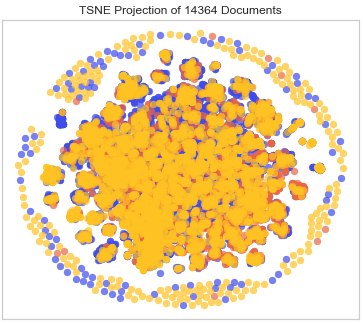
\includegraphics[width=\textwidth]{tsne_projection.png}
    \caption{t-sne visualization of seed data}
    \label{fig:t-sne}
\end{figure}

Even though there are some approaches to clustering high dimensional data, it generally is difficult to do so accurately. 
One of the explanations is the increased sparsity and the difficulty to distinguish between the distances 
of specific instances \citep{tomasev2014roleofhubness}. For these reasons, an unsupervised approach was not chosen.

However, labeled data is still needed to train supervised machine learning models for sentiment analysis. While manually labelling
all data might be the most accurate solution, it is associated with high costs \citep{miller2020activelearningapproaches}.
Hence, this thesis proposes the implementation of an Active Learner. With its support, a complete domain-specific corpus can be labeled while only relying on partial annotations \citep{park2015EfficientExtraction}.
As a result, a domain-specific labeled text corpus is created that can be used as input to different supervised machine learning algorithms.

\subsubsection{Active Learner Workflow}
The illustrated workflow in Figure 2 provides an overview of how an Active Learner works. 
To begin with, cleaned and pre-processed data needs to be available that can be used by the Active Learner. 
Furthermore, the Active Learner can also be trained with some initial training data, which is also referred to as the seed. 
By using clustering algorithms, the seed data can be selected and labeled methodologically, which allows the Active Learner to achieve 
higher accuracy faster when compared to randomly picking the initial seed data \citep{kang2004usingclusterbasedsampling}. All the unlabeled 
instances will become the pool data, which need to be labeled. The seed data is fed into the Active Learner and trains an estimator, 
which needs to be defined when creating the Active Learner.\\
In addition, a query strategy needs to be defined, based on which the Active Learner queries new instances from the aforementioned pool. 
A query strategy evaluates the informativeness of unlabeled samples. Common strategies are \emph{uncertainty sampling, query-by-committee, 
expected model change, expected error reduction and variance reduction}.\\
While each strategy has its own intricacies, all essentially try to find instances that are hard for the model to classify and hence might benefit from manual annotation. 
After the query function selected instances from the pool, an oracle needs to label those. An oracle normally is at 
least one human with knowledge on how to annotate the data at hand \citep{settles2009activeLL}. Once the new instances are labeled, 
those instances need to be removed from the pool, since they are now part of the labeled data. The Active Learner then needs 
to be taught the new instances, which he can use to adjust the model. After each iteration, the results can be evaluated. 
A common performance measure for Active Learners is \emph{accuracy}.\\
If a predefined stopping criterion is not yet met, the query strategy selects more instances from the pool and repeats the process.
If the stopping criterion is met, the process ends \citep{lu2019investigating}.

\begin{figure}
    \centering
    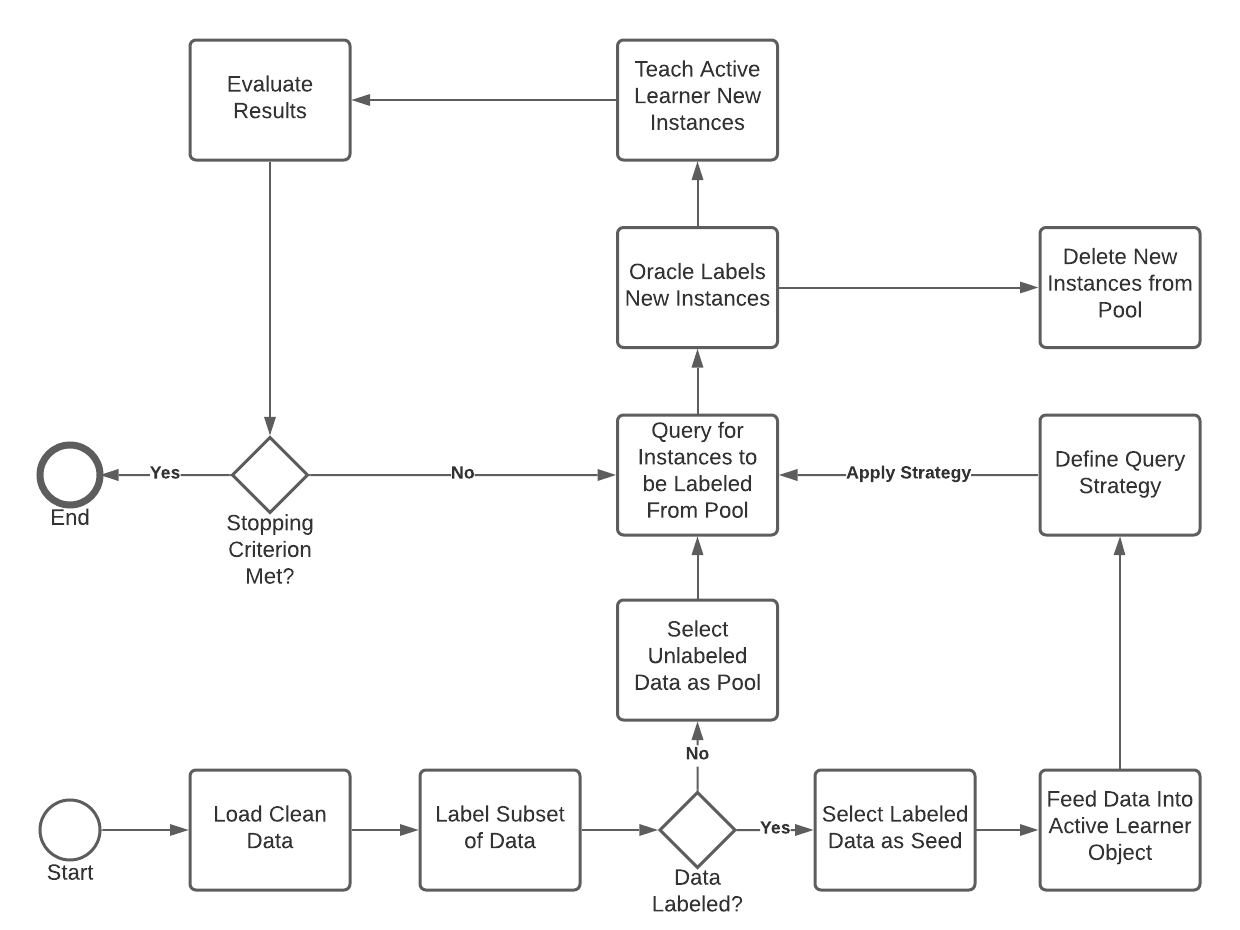
\includegraphics[width=\textwidth]{al_workflow.png}
    \caption{Visualized Workflow of an Active Learner. Created with lucid.app}
    \label{fig:AL_Workflow}
\end{figure}

\subsubsection{Sentiment Analysis Models}
The next sub-section explores the machine learning models that will be used to perform sentiment analysis on the domain-specific corpus created by the Active Learner. \\

\noindent\textbf{Naïve Bayes (NB)}\\
NB is a probabilistic supervised machine learning model. By working probabilistically, the classifier assigns the probability of 
belonging to a given class based on certain features \citep{jemai2021SentimentAnalysis}. Because of the high dimensionality of text data, 
which can be handled very well by NB, this algorithm has established itself as one of the standards for sentiment analysis. 
This thesis will use Multinomial Naïve Bayes (MNB) to classify the sentiment of the text. This is due to the model's ability to handle 
larger vocabulary sizes \citep{abbas2019mnb}. In addition, the algorithm is simple to implement, suitable for real-time applications, and highly scalable. 
However, the algorithm's prediction accuracy is frequently lower than that of other sentiment analysis techniques \citep{song2017novelclassification}. 
Due to the easy implementation and fast training of the algorithm, MNB will serve as the baseline classifier.\\

\noindent\textbf{Long Short Term Memory (LSTM)}\\
LSTMs are becoming increasingly popular for sentiment classification. 
LSTMs are built on a recurrent neural network architecture (RNN). In an RNN the neurons are connected to themselves through time. 
As a result, the input from a time instance t\textsubscript{i} will also be used as an input for the next time instance t\textsubscript{i+1}. That leads to the 
problem of vanishing gradients, which means that it is hard for the model to learn long-term dependencies. This occurs because
in a long sequence, like a sentence, as the loss gradients are backpropagated through the RNN, they may shrink to zero \citep{vanishinggradients2020pmlr}.
LSTMs are designed to overcome that problem.
The LSTM architecture does so via its four constituents: A memory cell which can remember a lot of information 
from previous states, an input gate which controls the inputs into the neurons, an output gate with an activation function 
and lastly a forget gate which resets the neuron \citep{priyantina2019sentimentanalysishotel}. When training an LSTM, it is shown that
using a pretrained Word2Vec embedding can help solving the curse of dimensionalty that might occur when using a one-hot encoded input \citep{xiao2018word2veclstm}.\\
%Hence, a Word2Vec embedding layer is used in the LSTM.

\noindent\textbf{Bidirectional Encoder Representations from Transformers (BERT)}\\
BERT is a relatively new machine learning algorithm developed by Google in 2018 and mainly designed for 
natural language processing. BERT is pretrained on the English Wikipedia and BooksCorpus. Because of the 
pretraining users won't need as much computing power to achieve good results, even if the dataset is relatively 
small \citep{devlin2019bert}. The BERT github page even states that 
“Most NLP researchers will never need to pre-train their own model from scratch” \citep{googlegithub}.\\

\noindent\textbf{Valence Aware Dictionary for sEntiment Reasoning (VADER)}\\
Due to widespread usage of lexicons, the VADER sentiment lexicon was also included. However, the results of VADER are intended for illustrative purposes only,
as a lexicon based approach is not within the research scope of this thesis.
VADER is specifically designed to classify social media sentiment and also includes emoticons, acronyms and \emph{slang} words \citep{hutto2015vader}. 
Vader looks up the associated compound score of words in the lexicon. Based on the score, the sentiment is determined.
The VADER lexicon does not have any hyperparameters to tune. It is only possible to optimize the classification results by
changing the thresholds of the score.

\subsubsection{Evaluation Metrics for Sentiment Classification}
Typically, \emph{accuracy, precision, recall and the F-score} are used as evaluation metrics to assess the performance of a sentiment analysis model. \\
\emph{Accuracy} is the percentage of correctly predicted observations over all instances. Accuracy should only be used if the classes in the data are balanced.
Otherwise, a model that only predicts the majority class may be able to achieve quite high accuracy.\\
\emph{Precision} expresses the proportion of how many classes were classified as positive, that actually are positive.\\
\emph{Recall} refers to the percentage of total relevant results that were correctly classified.\\
\emph{F-score} is a metric that combines precision and recall and presents the harmonic mean of the two \citep{hossin2015evaluationmetrics}.

\begin{equation*}
    Accuracy = \frac{TP+TN}{TP+FP+TN+FN}
\end{equation*}

\begin{equation*}
    Precision = \frac{TP}{TP+FP}
\end{equation*}

\begin{equation*}
    Recall = \frac{TP}{TP+TN}
\end{equation*}

\begin{equation*}
    F_{1}=\frac{2*(Precision * Recall)}{Precision + Recall}
\end{equation*}

\noindent In the formulas above, \emph{TP} and \emph{TN} are positive and negative classes that were correctly classified. Contrary, \emph{FP} and \emph{FN} are
incorrectly classified instances.\\
Even though the class distribution of the data used in this thesis is skewed towards to label \emph{bullish}, the remaining two classes still represent
almost 50\% of the data. As a result, accuracy can still lead to representative results, which is why this metric is used for hyperparameter tuning and model selection.

\subsubsection{Stock Price Prediction Models}
The next section explores the machine learning models that will be used to predict the stock price of GameStop. \\

\noindent\textbf{ARIMA}\\
One of the standard methods for time series forecasting is ARIMA. Therefore, it is commonly used in forecasting stock prices.
However, it has some limitations, especially with regards to modelling the non-linear relationships between variables. As a result,
some prerequisites are required to create good results \citep{sima2018timeseries}.
First of all, ARIMA does not work well with seasonal data. Seasonality can be identified by plotting the stock prices, Autocorrelation and Partial Autocorrelation.
Furthermore, ARIMA only works on stationary time-series. 
By differencing the time-series it can be made stationary and then be used in the ARIMA model.
The dickey fuller test can be used to test for stationarity \citep{jain2017ASO}.
If the null hypothesis of the test can be rejected, the time series is assumed to be stationary. \\

\noindent\textbf{LSTM without Other Features}\\
As stock prices are generally volatile, non-stationary and can have changes in their statistical properties it is beneficial to use
models that can learn those attributes. Since LSTMs are able to capture such contextual information, they are shown to outperform many other methods \citep{preeti2019lstm}.
This thesis implements a Vanilla LSTM, which is a model with only a single LSTM layer. This implementation was chosen because others, such as a stacked-LSTM, do not necessarily outperform a Vanilla LSTM for stock price prediction tasks \citep{hai2020lstms}.
Even though this thesis explores various hyperparameters for the Vanilla implementation, it does not explore other implementations as that would go
beyond the research-scope of the thesis.
When using an LSTM for time-series tasks, a look-back period needs to be defined which chooses how many previous timestamps, for the case at hand - days, will be used to predict the 
stock price at the next timestamp \citep{lim2020lookback}.\\

\noindent\textbf{LSTM with Other Features}\\
One advantage of LSTMs is that they can also include other features into their time-series prediction.
When including other input features in addtition to the stock price, the time series is considered to be multivariate \citep{liu2019multivariate}.
To answer the research question outlined in the \nameref{introduction}, the obtained sentiment was added as an input feature to the model. However, since the literature
also identified other features, besides sentiment, as strong predictors this thesis will also explore the performance of a model that only includes trading volume.

\subsubsection{Evaluation Metrics for Stock Price Prediction}
Standard evaluation metrics for time-series data include Mean Absolute Error (MAE), Mean Squared Error (MSE) and Root Mean Squared Error (RMSE) \citep{rezaei2021stockpriceprediction}.\\
\emph{MAE} computes the absolute difference between the actual and predicted price. As a result, the MAE is on the same unit scale as
the output value.\\
\emph{MSE} represents the squared distance betwen the actual and predicted prices. \\
\emph{RMSE} simply takes the square-root of MSE. Hence, the output value is the same unit as the required output and can still represent the
dispersion of results. Therefore, RMSE will be used as the evaluation metric to select the best hyperparameters and model.
In the formulas $y_{i}$ represents the actual value and $\hat{y}_i$ the predicted value \citep{chen2021meanvariance}.
The aforementioned metrics are defined as follows:

\begin{equation*}
    MAE = \frac{1}{n}\sum_{i=1}^{n}|y_{i}-\hat{y}_{i}|
\end{equation*}

\begin{equation*}
    MSE = \frac{1}{n}\sum_{i=1}^{n}(y_{i}-\hat{y}_{i})^2
\end{equation*}

\begin{equation*}
    RMSE = \sqrt{\frac{1}{n}\sum_{i=1}^{n}(y_{i}-\hat{y}_{i})^2}
\end{equation*}


\subsection{Experimental Setup}
The following subsection will explore how the methods outlined in the \nameref{general_description} were implemented.
All the code was written in Python version 3.9.7 in the Visual Studio Code IDE. All the packages that were installed in the 
virtual development environment of this thesis can be found in \nameref{appendix:A}.

\subsubsection{Data}

\noindent\textbf{Reddit Posts}\\
While Reddit does offer an official API, the API is most useful for streaming data. 
There are some strict limitations on accessing large amounts of historical data. As a result, the official API is not the best choice for this thesis. 
However, \emph{pushshift.io} provides a solution for the strict limits. Essentially, Pushshift copies data from Reddit at the time it is posted. Since Pushshift uses the document-based database Elastic, it is extremely fast to query data \citep{elastic2015}.
To access Pushshift, this thesis uses an API wrapper called \emph{PMAW}. Since requests are I/O-bound, PMAW is multithreaded. Hence, requests can be run asynchronously which allows the data to be loaded much faster \citep{pmaw2021}.

For this thesis all Gamestop (GME) related posts between January 1st, 2020 and October 26th, 2021 were requested for the subreddit WallStreetBets. 
The query returns 89 columns. Most of which, however, can be dropped since they either are not useful for this thesis or contain no data. 
The most important columns are the title and the content of the post. 
Emoticons are also included in the content text. In total 179,544 posts were obtained. Of all obtained posts, 10\% or 17,955 were manually labeled as either bearish, neutral or bullish. This was done by using a graphical user interface that displayed the title and
text of every tenth Reddit post. Of all manually labeled data 3479 (19.4\%) are bearish, 5119 (28.5\%) are neutral and 9357 (52.1\%) are bullish. \\

\noindent\textbf{GameStop Stock Price}\\
By using the python library yfinance, stock prices for GameStop can easily be obtained from Yahoo Finance. The start and end dates are the same as the ones used to load data from Reddit.
By loading the data, the columns Date, Open, High, Low, Close, Adjusted Close and Volume are returned. This thesis only uses the Date, Volume and Adjusted Close, which is the closing price
of the stock after adjusting for factors such as dividend payouts.

\subsubsection{Active Learner Implementation}
To implement an Active Learner the \emph{modAL} package was used. modAL was designed with modularity, flexibility and extensibility as high priorities \citep{danka2018modal}. 
The estimator defined in the Active Learner object is a \emph{Support Vector Machine (SVM)}. A SVM was chosen because of its strong generalization 
performance \citep{alves2014comparisonsvm}.
For the case at hand, the algorithm needs to solve a classification problem by optimally separating the data between bearish, 
neutral and bullish instances. Classification is done by fitting a hyper-plane with the biggest margin, meaning it looks for the greatest distance 
to the nearest sample points \citep{jemai2021SentimentAnalysis}. SVMs use spatial transformations, commonly known as kernel functions, to fit the hyperplane.
By doing so the data is projected into a higher dimensional space, which makes them easier to separate.
Kernels can be linear, RBF or others. The radial basis function (RBF) kernel is best used for non-linear problems and is a general-purpose kernel that 
is often used in pattern recognition problems. The linear kernel, on the other hand, is typically used when there are only two classes present. 
A good example for that might be positive and negative sentiment \citep{alves2014comparisonsvm}.

The initial seed data to train the SVM-estimator in the Active Learner was the data that was annotated manually.
Since an SVM cannot handle text data, the data had to be preprocessed and converted to a tf-idf representation. % Explain tf-idf representation
Furthermore, the implementation of the Active Learner in this thesis deviates from the literature a little bit: The literature that was reviewed
does not set aside a test set from the initial seed data and the accuracy of the Active Learner is evaluated on the entire seed data after every iteration. 
While the literature does not explain why this approach was
taken, I hypothesize that is due to the cost associated with labeling the data. This thesis will not deviate from well established machine learning practices
and therefore set aside 20\% of the seed data as test data, which will be used to evaluate the performance of the Active Learner after every iteration \cite[p. 196]{raschka2019pythonmachinelearning}.

Uncertainty sampling was chosen as the query strategy because it has been demonstrated to be a strong baseline strategy. 
This query strategy assumes, that instances that are far from the decision boundary are adequately explainable and instances close to the 
decision boundary are uncertain. Naturally, this complements the SVM-estimator very well. As a result, the Active Learner queries 
the samples about which it is most uncertain about \citep{osbonre2004ensemblebased}. Two human oracles labeled an additional 10\% of the data,
which were chosen by the Active Learner. Those 10\% were chosen by the Active Learner in ten iterations, meaning the Active Learner loop was repeated
every time an additional 1\% of the data was labeled. Subsequently, the estimator was retrained on all labeled instances, excluding the test set.

\subsubsection{Data Preprocessing}
The research by \cite{jemai2021SentimentAnalysis} presents a system for structuring a sentiment analysis project, which was also applied in this thesis.
The data collection phase is the first step, where textual data is obtained from a source. 
The data is then cleaned in the second step, the data pre-processing phase. To do so, several actions need to be performed.
One of them is tokenization. This is a natural language processing technique in which a large body of text is broken down into multiple sentences, 
each of which is then broken down into a list of words. Stop words such as is, the, a and other common words are also removed during the 
pre-processing phase. If stop words are included, they may play a negative role in sentiment classification and increase the overall 
vocabulary size while having little predictive power. \citep{zhao2017comparisontextprocess}.
In addition, special characters such as @ and urls should also be removed. 
It is also suggested that the text is converted to lowercase. As the final step, the research proposes lemmatization. By doing so,
the structure of a word is analyzed and converted to its normalized form. The research conducted by \cite{camachocollados2018role} 
shows that lemmatization improves sentiment analysis results especially when using domain-specific datasets.

Since it is shown that having data with emoticons leads to more accurate results than data without emoticons,
this thesis does not remove emoticons from the text corpus \citep{parveen2016sentimentanalysistwitter}.

\subsubsection{Sentiment Analysis Models Implementation}
The next section explores how the machine learning models to classify sentiment were implemented and how their optimal hyperparameters were chosen.
Before training the models, 20\% of the data were set aside as the test set. By setting aside 20\% of the training data as a validation set 
the optimal hyperparameters were selected. To account for class imbalances, stratification was applied. As a result, the sets have approximately the same
class distribution as the full set \citep{sahu2017stratification}.
Stratification was chosen over other methods to handle class imbalances, such as over- or undersampling, because the imbalance
is not too extreme \citep{ganganwar2012overview}.\\

\noindent\textbf{Multinomial Naïve Bayes (MNB)}\\
To train the classifier, the data was first converted to a tf-idf representation.
The classifier uses five-fold gridsearch cross-validation to find the optimal parameters for
\emph{fit\char`_prior}, which determines if prior class probabilities shall be learned, and \emph{alpha}, which is a smoothing parameter that solves
the problem of zero probability. That problem might occur, if a an unseen word appears in the test set. By setting alpha to a value greater than
zero, the model pretends to have seen a word before.\\

\noindent\textbf{Long Short Term Memory (LSTM)}\\
Before training the LSTM, data is first fed into a Word2Vec model to learn the word embeddings. As explained in the literature, this can enhance the performance of the model by learning the similarity between words.
Selecting optimal hyperparameters for the Word2Vec model is oftentimes neglected, even though that may lead to performance differences.
The Word2Vec hyperparameters that were analyzed is the \emph{vector\_size, min\_count} and \emph{window}. The optimal respective hyperparameters are 50, 1 and 1. Those were determined based on a comparative intrinsic evaluation \citep{schnabel2015embeddings}.
A subset of the most similar words, calculated as the cosine similarity, of given words can be found in \nameref{appendix:B}.
The input and output dimensions of the Embedding layer of the LSTM, as well as the weights are taken from the word2vec model.
The output dimensions of the embedding layer are also used as the units for the subsequent LSTM layer. Furthermore, the model adds a Dropout layer to improve generalization. To find the optimal dropout parameter and optimizer for the model,
a loop runs through a set of parameters when fitting the model. The optimal model is determined by evaluating the performance on the validation set, which is 20\% of the training data. 
The final Dense output layer uses softmax as its activation function. Furthermore, the model uses categorical crossentropy as its cost function and accuracy as its metric.\\

\noindent\textbf{Bidirectional Encoder Representations from Transformers (BERT)}\\
To train BERT, the token \emph{[CLS]} and \emph{[SEP]} are added to the beginning and end of the input sequence. Subsequently, the tokens are converted to IDs using the tokenization
module from the bert library. Even though a maximum of 512 tokens can be used when training BERT, this implementation only uses a maximum of 100 tokens due to computational reasons.
Furthermore, this implementation uses an Adam optimizer and a constant learning rate of 0.00001. Future work should include an optimization of those parameters. The model is trained with
a batch size of two over three epochs. Write about hyperparameter tuning.\\

\noindent\textbf{Valence Aware Dictionary for sEntiment Reasoning (VADER)}\\
Typical threshold values for the obtained compound score are as follows: 
If the score is greater than or equal to 0.05, it is associated with positive sentiment. If the score is smaller than or equal to -0.05 it is associated with negative sentiment. For scores
in between, neutral sentiment is assigned \citep{hutto2015vader}. To obtain optimal evaluation metrics, however, the thresholds 0.03, 0.05, 0.07 and 0.10 and their negative counterparts were
also analyzed.

\subsubsection{Stock Price Prediction Implementation}
When splitting time series data, it needs to be split into windows. The training set consists of the first 80\% of the timeseries data and
the test set of the remainding 20\% of the data. To select the optimal hyperparameters, a rolling forecast is implemented. By doing so, the model 
sequentially adds the most recent observation and then rebuilds the model \citep{sima2018timeseries}.\\

\noindent\textbf{ARIMA}\\
% https://stats.stackexchange.com/questions/394796/should-my-time-series-be-stationary-to-use-arima-model
First the stock price data was analyzed to identify a seasonality pattern and to check for stationarity.
By visualizing the stock price, no seasonality was identified. This makes sense, because the data does not contain many years.
As a result, 
After differencing the time-series once the dickey-fuller test was applied, which showed stationarity at the 1\% significance level.
The hyperparameters that can be optimized are the number of lag observations
included in the model (p), the number of times the data needs to be differenced (d) and the size of the moving average window (q) \citep{sima2018timeseries}. As a result the following
hyperparameters were used: (5,0,0), (1,0,1), (2,0,2), (0,0,5), (1,0,0), (0,0,1), (0,0,0). \\

\noindent\textbf{LSTM without Other Features}\\
The data fed into the LSTM, in comparison to the ARIMA model, was not differentiated as one of the strengths of an LSTM is that it can also work well with non-stationary data.
As the first step, the input data was scaled to be between 0 and 1. This is standard practice and commonly applied in the literature. As a result, the LSTM is expected to be
less sensitive to the scale of the input data.
The LSTM looks for the optimal hyperparameters of the optimizer, the lookback period, and the dropout on the input which excludes a random subset of the data from the node activation and update of the weights.
A lookback period between one and five days was chosen, because \cite{saud2020lookback} found that a suitable lookback period for LSTMs is less than 5. \\

\noindent\textbf{LSTM with Other Features}\\
The LSTM model that includes other features uses the same hyperparameters as the model without sentiment. The only difference is
that sentiment or trading volume are also included as scaled input features.
For the model that also includes sentiment, however, some additional preprocessing steps were required. That is because sentiment is measured for every post, of which there
can be multiple per day, whereas there is only one time-series observation per day.
Therefore, sentiment was encoded as -1 for bearish, 0 for neutral and 1 for bullish. Then the sentiment was summed up and added
to the relevant date. 
By doing so, the collective sentiment of the entire WallStreetBets forum on a given day can be included. If, for example, more people are bullish that should lead to higher stock prices.
Whereas, if more people are less optimistic about the stock, that should lead to lower stock prices.

% End Method ----

% Begin Results ----

\section{Results}

This section is broken down into three parts. First the Active Learner results are looked at, then the sentiment models and
lastly the stock price prediction models. If the visualization uses a horizontal bar chart, the best result is the one on top.
If the visualization contains multiple line charts, the best result is a solid line and the rest a dashed line.

\subsection{Active Learner Results}
The Active Learner is represented as  a line chart with the accuracy on the y-axis and the respective query instance on the x-axis.
The accuracy at query-instance 0 is the performance after the initial training on the seed data.
As can be seen in Figure \ref{fig:ActiveLearner}, the performance of the Active Learner hit a plateau relatively quickly. It is hypothesized that
this plateau was reached for two reasons: First, by labelling the data at the document level, a document can contain bearish, neutral
and bullish words. Those contradictions may not only make it hard for the model to learn the structure of the input, but also for 
the human annotator when labeling the data. Additionally, by having two different human oracles to label the data, inconsistencies
may occur.

\begin{figure}
    \centering
    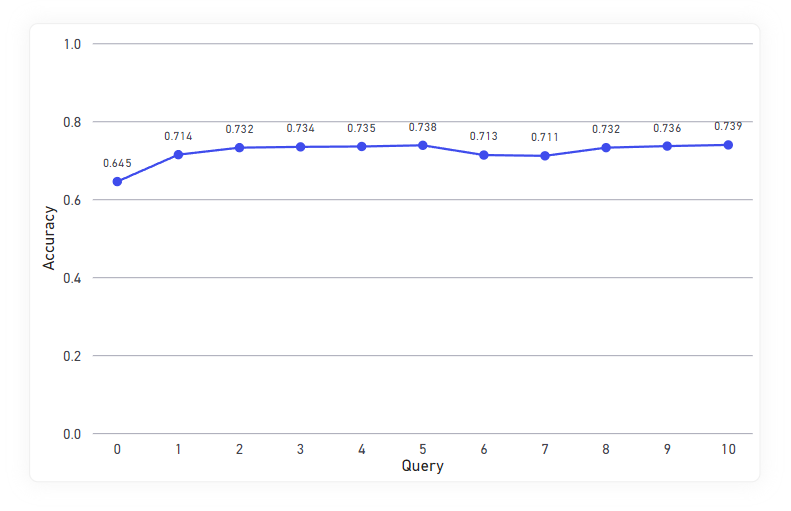
\includegraphics[width=\textwidth]{ActiveLearner.png}
    \caption{Accuracy of Active Learner over 10 query instances}
    \label{fig:ActiveLearner}
\end{figure}

\subsection{Sentiment Models Results}
The best performing model is selected based on the validation set and will subsequently be used to determine the sentiment for the
rest of the dataset. The best performing hyperparameter-set of the NB classifier achieved accuracy of 0.80, the LSTM 0.89 and BERT XYZ. \\

\noindent\textbf{MNB}\\
Since the Naive Bayes model does not train over epochs, its results are visualized on a bar chart. As can be seen in Figure \ref{fig:nb_hyperparam} the
highest accuracy of 80.4\% can be achieved by setting the hyperparameters alpha to one and fit\_prior to False. This baseline estimator
performs much better, than just randomly guessing the majority class (bullish). \\

\begin{figure}[!htb]
    \centering
    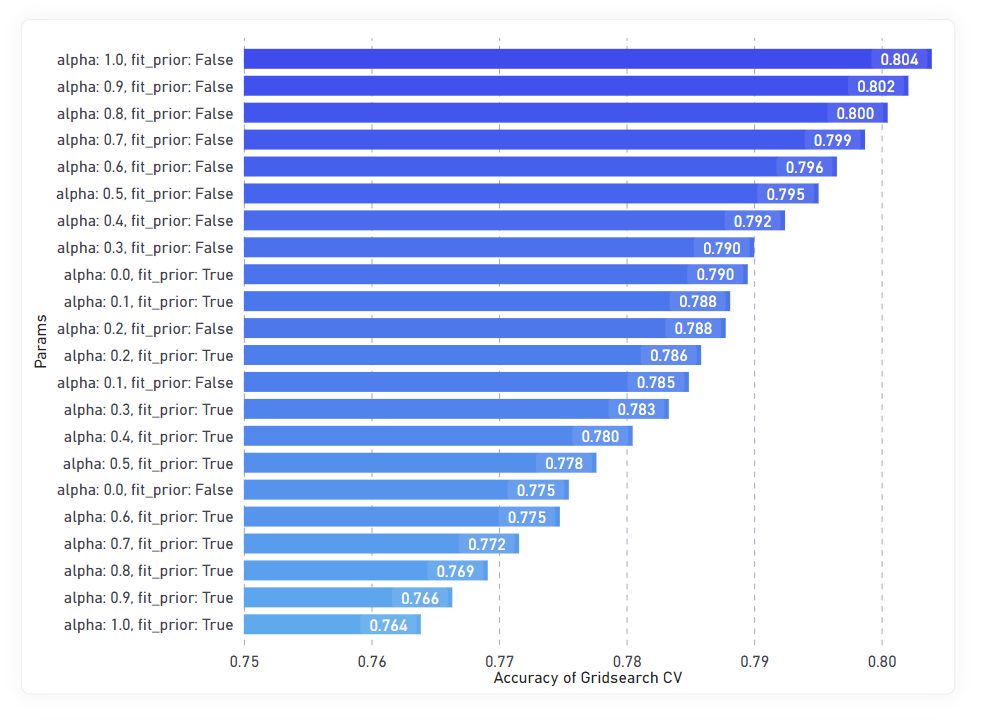
\includegraphics[scale=0.5]{NB_hyperparam.png}
    \caption{Accuracy of NB With Varying Hyperparameters}
    \label{fig:nb_hyperparam}
\end{figure}


\noindent\textbf{LSTM}\\
The LSTM finds its optimal hyperparameters after three epochs, after which it seems to start overfitting a little bit.
This can be concluded, as the valuation set accuracy in Figure \ref{fig:lstm_acc_loss} starts dropping, while the training set
accuracy keeps improving. The same can be concluded for the loss as visualized in Figure.
The optimal hyperparameters are a dropout rate of zero and the Adam optimizer.\\

\noindent\textbf{BERT}\\
Since BERT is already pre-trained, it does not need as many epochs to optimize a model.
As can be seen in figure ABC, there is almost no change to the accuracy, meaning the model does not benefit from training over more epochs.
To be continued.

\begin{figure}
    \centering
    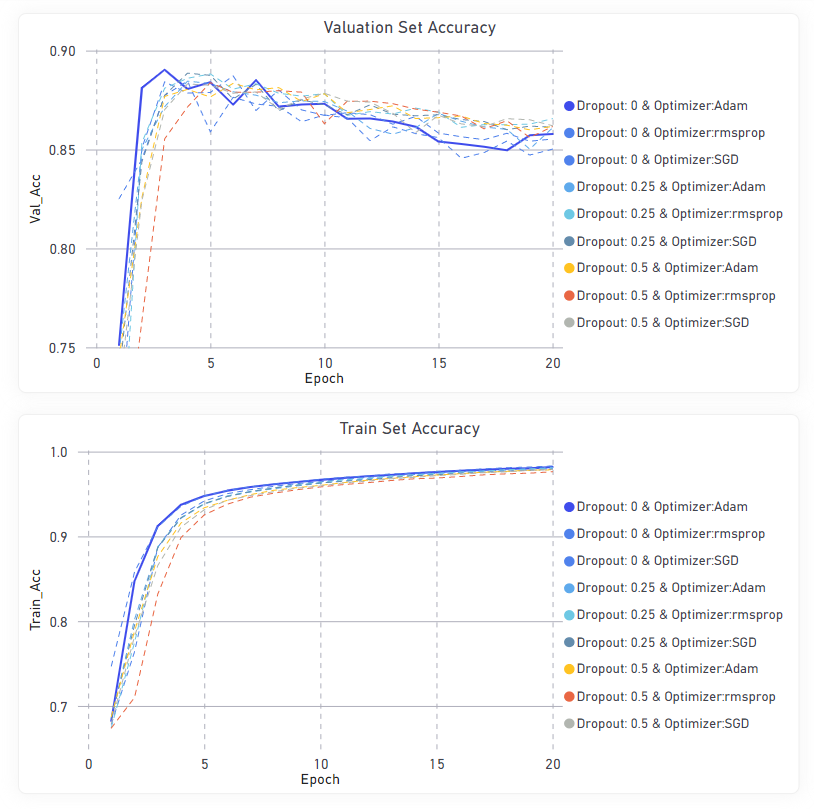
\includegraphics[scale=0.55]{LSTM_Accuracy.png}
    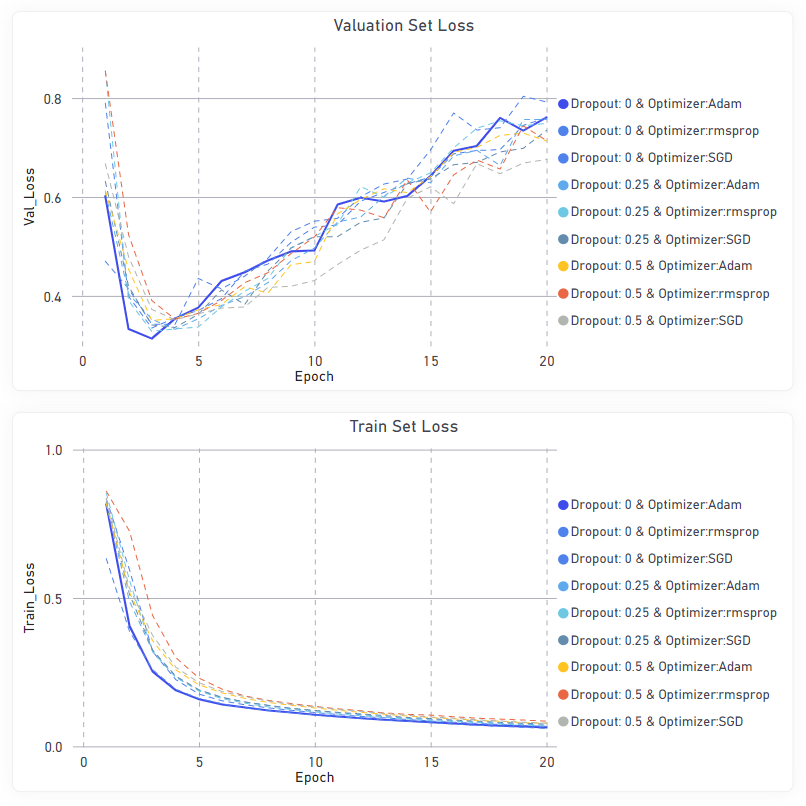
\includegraphics[scale=0.55]{LSTM_Loss.png}
    \caption{Accuracy and Loss of LSTM-Classifier with Varying Hyperparameters}
    \label{fig:lstm_acc_loss}
\end{figure}


\subsubsection{Write later about Test set}
Based on that the ABC classifier was chosen to label the rest of the data. To compare how well the models generalize, the evaluation metrics
of the testsets are outlined in Table \ref{tab:results}. As can be seen the commonly used VADER lexicon underperforms the NB baseline model by a big margin.
The deep learning models, however, show quite strong results even though they overfit quite a bit.

\begin{table}[!htb]
    \caption{Test Set Evaluation Metrics for NB, LSTM and BERT - Needs to be updated!}
    \label{tab:results}
    \centering
    \small

    \begin{tabular}{lllrr}
        \toprule
                                        & \multicolumn{4}{c}{Evaluation Metrics} \\
                                        \cmidrule{2-5}
                            Model       & Accuracy      & Precision     & Recall    & F\textsubscript{1}-Score \\
            \midrule
            \multirow{1}{*}{NB}         & \textbf{0.79}          & \textbf{0.74}          & \textbf{0.82}      & \textbf{0.76}                      \\
            \midrule
            \multirow{1}{*}{LSTM}       & 0.50          & 0.53          & 0.53      & 0.53                      \\
            \midrule
            \multirow{1}{*}{BERT}       & 0.52          & 0.17          & 0.33      & 0.23                      \\
            \midrule
            \multirow{1}{*}{VADER}      & 0.39          & 0.38          & 0.39      & 0.38                      \\

        \bottomrule
    \end{tabular}

\end{table}
\pagebreak
\pagebreak
\subsection{Stock Prediction Results}
The best performing stock price prediction model and its hyperparameters was selected based on the RMSE of the validation set. As can be seen
in Table \ref{tab:results_stocks_valset}, the LSTM that only used Price as its input feature achieved the lowest RMSE for a given set of hyperparameters.

\begin{table}[!htb]
    \caption{Validation Set RMSE for ARIMA and LSTM Time-Series Models}
    \label{tab:results_stocks_valset}
    \centering
    \small

    \begin{tabular}{lllrr}
        \toprule                                        
                            Model       & RMSE  \\
            \midrule
            \multirow{1}{*}{ARIMA}         & 22.227  \\
            \midrule
            \multirow{1}{*}{LSTM including Price, Trading Volume and Sentiment}       & 0.087   \\
            \midrule
            \multirow{1}{*}{LSTM including Price and Sentiment}       & 0.084   \\
            \midrule
            \multirow{1}{*}{LSTM including Price and Trading Volume}      & 0.070    \\
            \midrule
            \multirow{1}{*}{LSTM that only includes Price}      & \textbf{0.061} \\

        \bottomrule
    \end{tabular}

\end{table}

Figure \ref{fig:lstm_models_rmse_loss} shows the RMSE and Loss for each LSTM model's respective input features with their optimal hyperparameter setting.
Even though on the validation set all models seem to flatten out eventually, the visualizations of the training set indicate that the model hasn't finished
learning its optimal weights yet and more epochs may be benefitial.

The RMSE and Loss of the best performing model on the validation set are presented in Figure \ref{fig:lstm_price_rmse_loss}. As can be seen, the lowest loss can be achieved
at epoch 28 with the hyperparameter setting Dropout equals zero, an Adam optimizer and lookback equals one. Since too many hyperparameters
were analyzed, only the five best performing ones were visualized. The RMSE and Loss for the models with other input features can 
be found in \nameref{appendix:Graphics}.
Because ARIMA is not trained over epochs, it is visualized as a bar-chart in Figure \ref{fig:arima_rmse}. As can be seen, the optimal hyperparameter setting is (0, 0, 1).

\begin{figure}
    \centering
    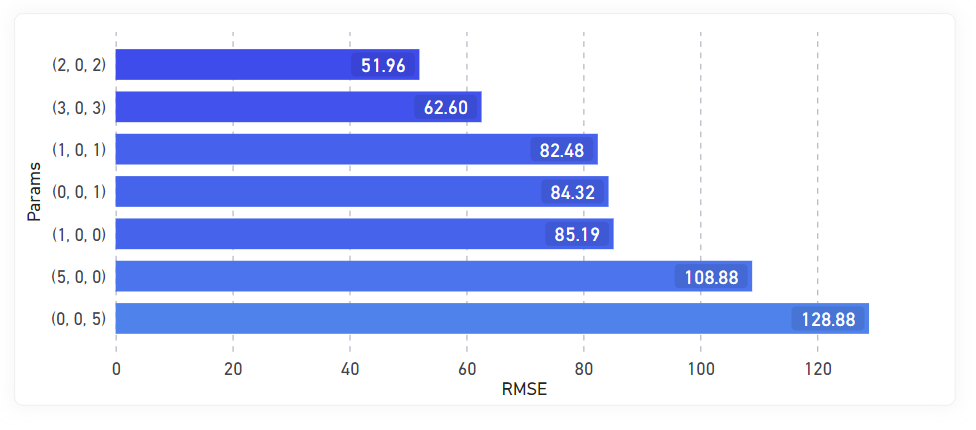
\includegraphics[width=\textwidth]{ARIMA_RMSE.png}
    \caption{RMSE of ARIMA}
    \label{fig:arima_rmse}
\end{figure}

\begin{figure}
    \centering
    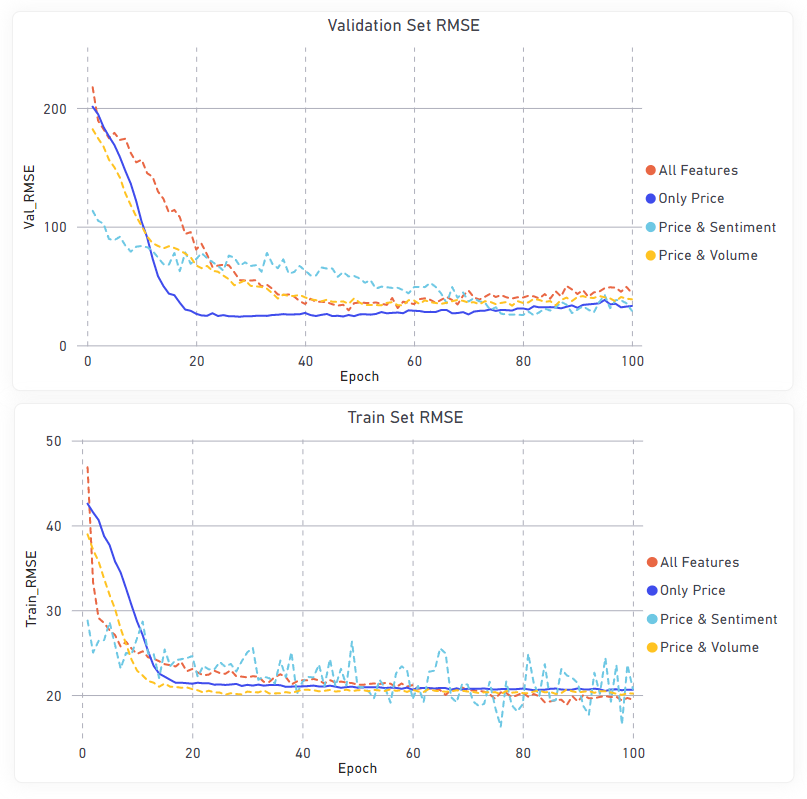
\includegraphics[scale = 0.55]{Best_Params_Of_Model_RMSE.png}
    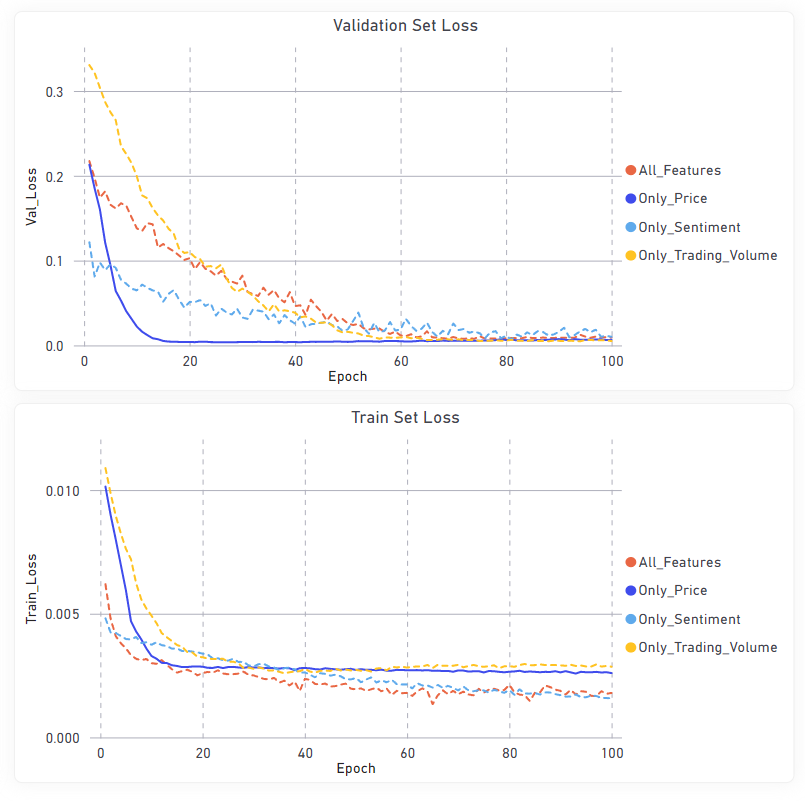
\includegraphics[scale = 0.55]{Best_Params_Of_Model_Loss.png}
    \caption{RMSE and Loss of Models with Various Input Features and Their Optimal Hyperparameters}
    \label{fig:lstm_models_rmse_loss}
\end{figure}

\begin{figure}
    \centering
    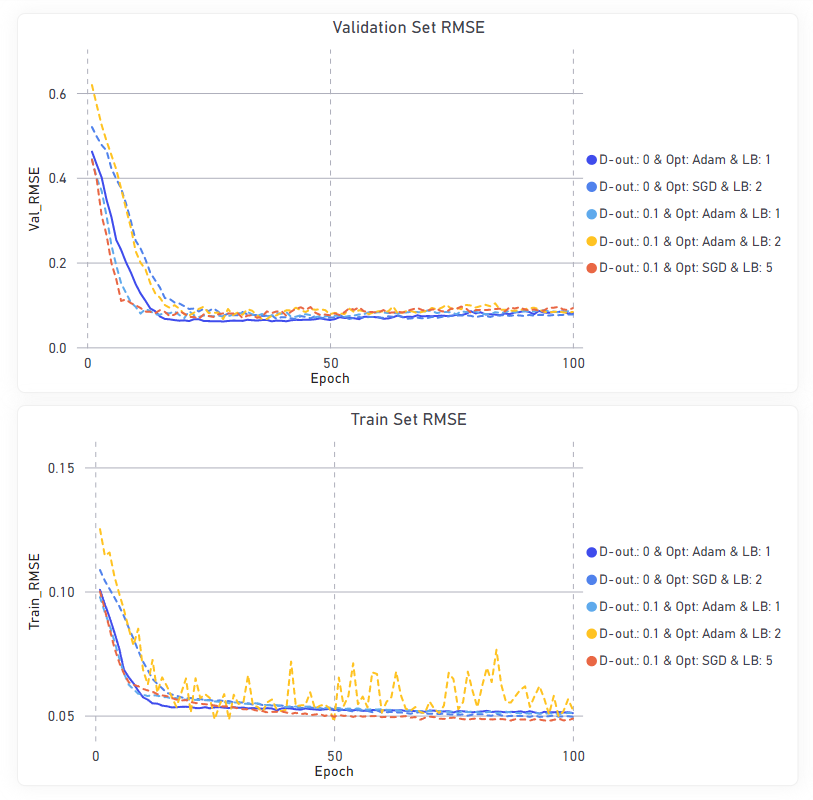
\includegraphics[scale = 0.55]{Only_Price_Params_RMSE.png}
    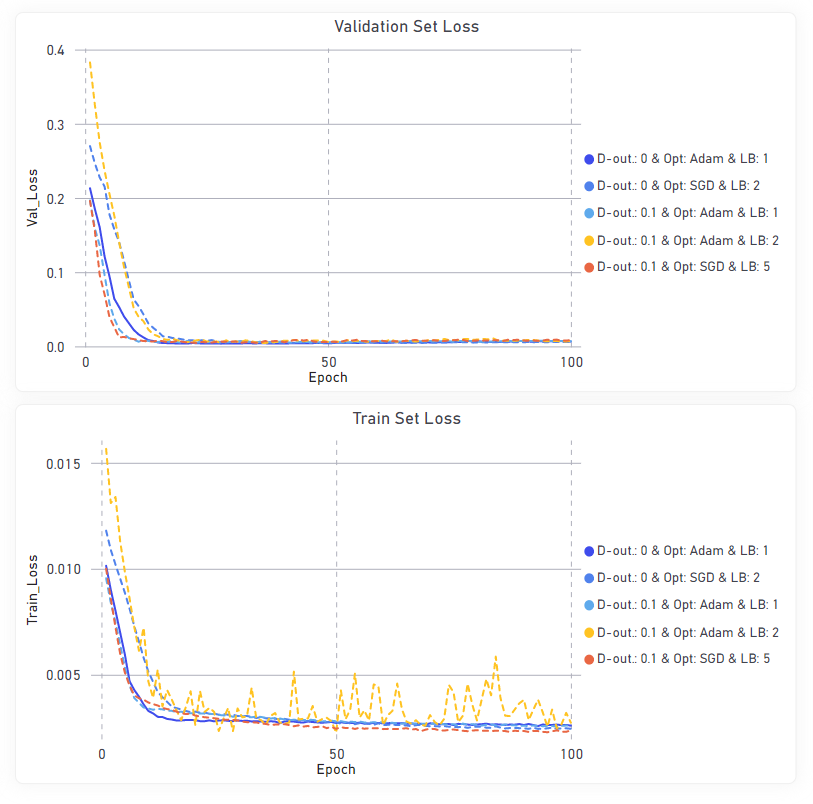
\includegraphics[scale = 0.55]{Only_Price_Params_Loss.png}
    \caption{Five Optimal Hyperparameters of LSTM Model With Only Price as Input Feature}
    \label{fig:lstm_price_rmse_loss}
\end{figure}


To see how well the different stock price prediction models generalize, they were evaluated based on their test set.
While all models seem to overfit quite a lot, the results of the LSTM models still seem promising. On the test set, however,
the model that includes price and trading volume seems to achieve the best performance. However, models shall always be selected
by their training set, which is why the model that only includes price shall be used. On the test set, it only ranks slighly worse
than the best performing model.

\begin{table}
    \caption{Test Set Evaluation Metrics for ARIMA and LSTM Time-Series Models}
    \label{tab:results_stocks}
    \centering
    \small

    \begin{tabular}{lllrr}
        \toprule
                                        & \multicolumn{3}{c}{Evaluation Metrics} \\
                                        \cmidrule{2-4}
                            Model       & RMSE      & MSE     & MAE    \\
            \midrule
            \multirow{1}{*}{ARIMA}         & 187.3          & 35,071.2          & 186.2 \\
            \midrule
            \multirow{1}{*}{LSTM including Price, Trading Volume and Sentiment}       & 14.0          & 196.8          & 11.3 \\
            \midrule
            \multirow{1}{*}{LSTM including Price and Sentiment}       & 9.2          & 84.3          & 6.5 \\
            \midrule
            \multirow{1}{*}{LSTM including Price and Trading Volume}      & \textbf{7.9}           & \textbf{63.0}          & \textbf{5.5} \\
            \midrule
            \multirow{1}{*}{LSTM that only includes Price}      & 8.5         & 71.7          & 6.4 \\

        \bottomrule
    \end{tabular}

\end{table}

As the plot of the predition of the test set in Figure \ref{fig:price_forecast_best_model}, it can be seen that the model does a fairly good job at predicting prices.
The price forecasts of the other models are represented in \nameref{appendix:Forecast}.

\begin{figure}[!htb]
    \centering
    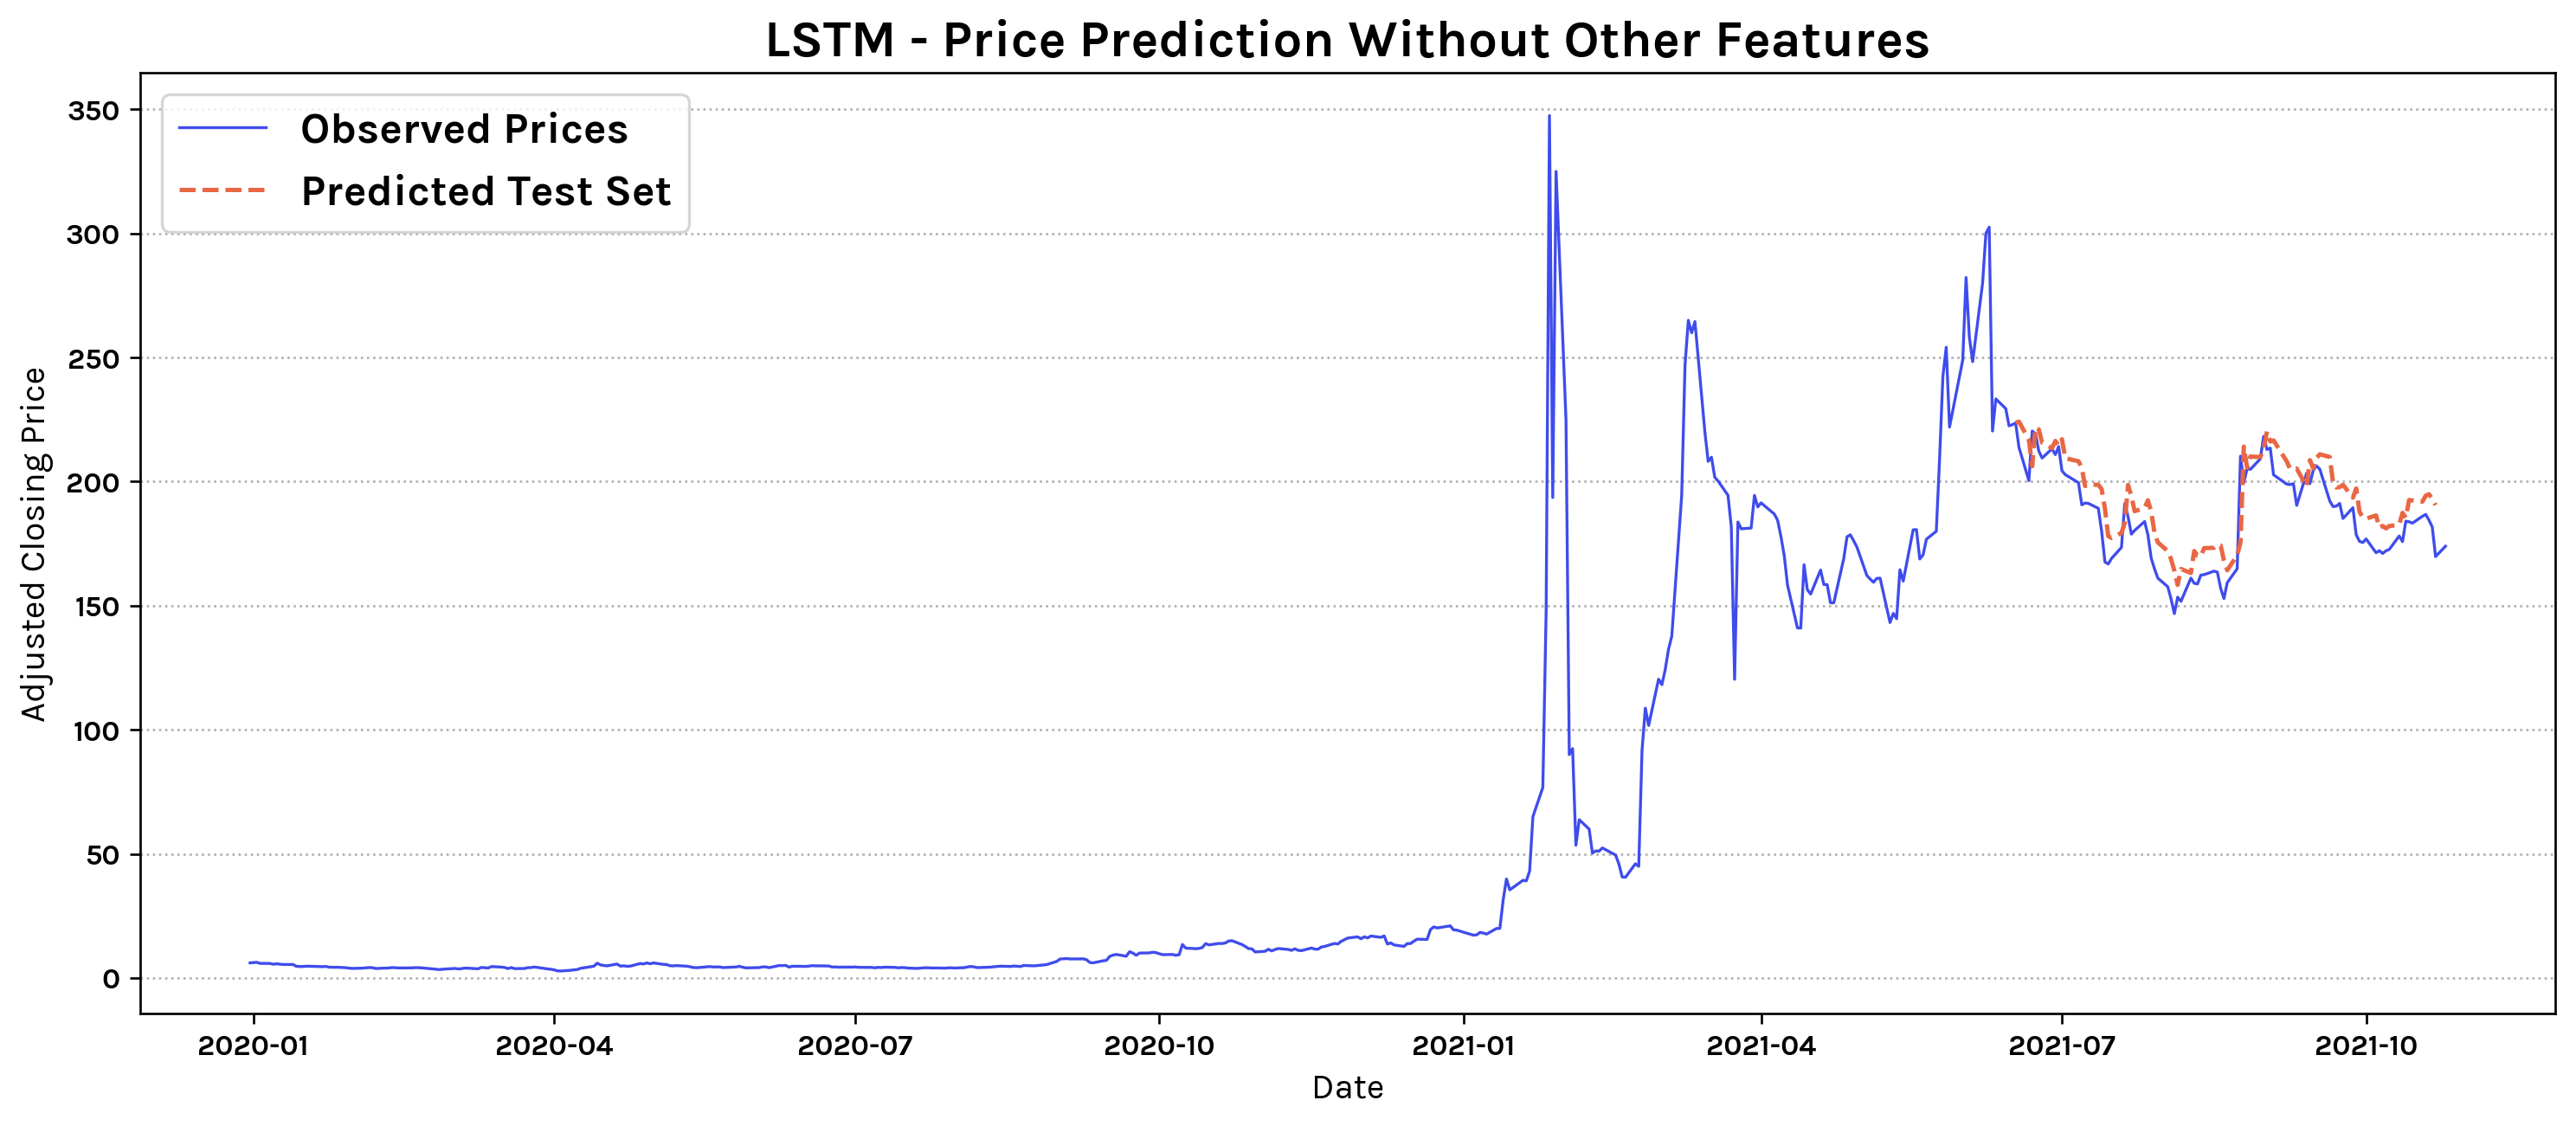
\includegraphics[scale=0.4]{no_other_feature_pred.png}
    \caption{Price Forecast of Selected Model from Validation Set}
    \label{fig:price_forecast_best_model}
\end{figure}

% End Results ----

% Begin Discussion ----

\section{Discussion}

The 'to the moon' WallStreetBets movement had a tremendous impact on the lives of individuals, both to the positive and negative. 
Besides that, however, many investment funds have also been negatively impacted by the recent short-squeezes. 
While it might seem noble to root for individuals who try to force large funds out of their positions at big losses, it is easy to forget that many 
of those funds manage money for charitable endowments, pensions and others. 
Furthermore, such disruptions to the financial markets can harm its stability, thus causing spillover effects which can also negatively impact the 
lives of many people \citep{lyocsa2021yolotrading}.
By being able to accurately measure and monitor the sentiment on WallStreetBets, market participants and regulators are able to preemptively take measures.\\
However, since the wallstreetbets subreddit has become very popular just recently, there is little academic research about the impact of the community on 
financial markets so far. Even though there is some research about sentiment analysis on wallstreetbets, that research does not use state of the art algorithms to perform 
sentiment analysis. This thesis shows that the wide-spread use of lexicons is not the best way to monitor sentiment and the adaption of better algorithms is urgently needed.\\
Not only did this thesis compare the performance of different models, but also proposed a highly efficient and reliable way to create a domain-specific annotated corpus, 
which can be used as the input to aforementioned models. To my knowledge, this thesis is the first research that creates a domain-specific corpus for the WallStreetBets forum. 
Researchers, such as \cite{talamas2021socialmediaeffectsonthemarket}, specifically propose future work on “inclusion of features derived from alternative manipulation of the data like sentiment analysis 
could lead to new insights“. I strongly believe that the methods proposed in my thesis lead to better sentiment classifiers, 
which can then be used in other scientific or industrial applications.

% End Discussion ----

% Begin Conclusion ----

\section{Conclusion}
This thesis proposes the use of an Active Learner to drastically reduce the total cost of annotation. 
As a result, it becomes more feasible to create a fully labeled domain-specific dataset. 
Once a fully labeled dataset is obtained, it can be used in supervised learning algorithms. 
The results show that using state of the art models underperform the simple baseline NB classifier.

% End Conclusion ----

\bibliography{references}

\section{Appendices}

\subsection{Appendix A}
\label{appendix:A}
List of packages used.

\subsection{Appendix B}
\label{appendix:B}

Example of the similarity (denoted in the parentheses) of the three most similar words of an input word: \\
robinhood -> rh (0.98), etrade (0.87), webull (0.86) \\
andromeda -> jupiter (0.95), mars (0.94), uranus (0.93) \\
ape -> autist (0.94), monkey (0.91), retard (0.90) \\
hedgefund -> hfs (0.93), hf (0.89), shorter (0.88) \\

\subsection{Appendix Graphics}
\label{appendix:Graphics}

\begin{figure}
    \centering
    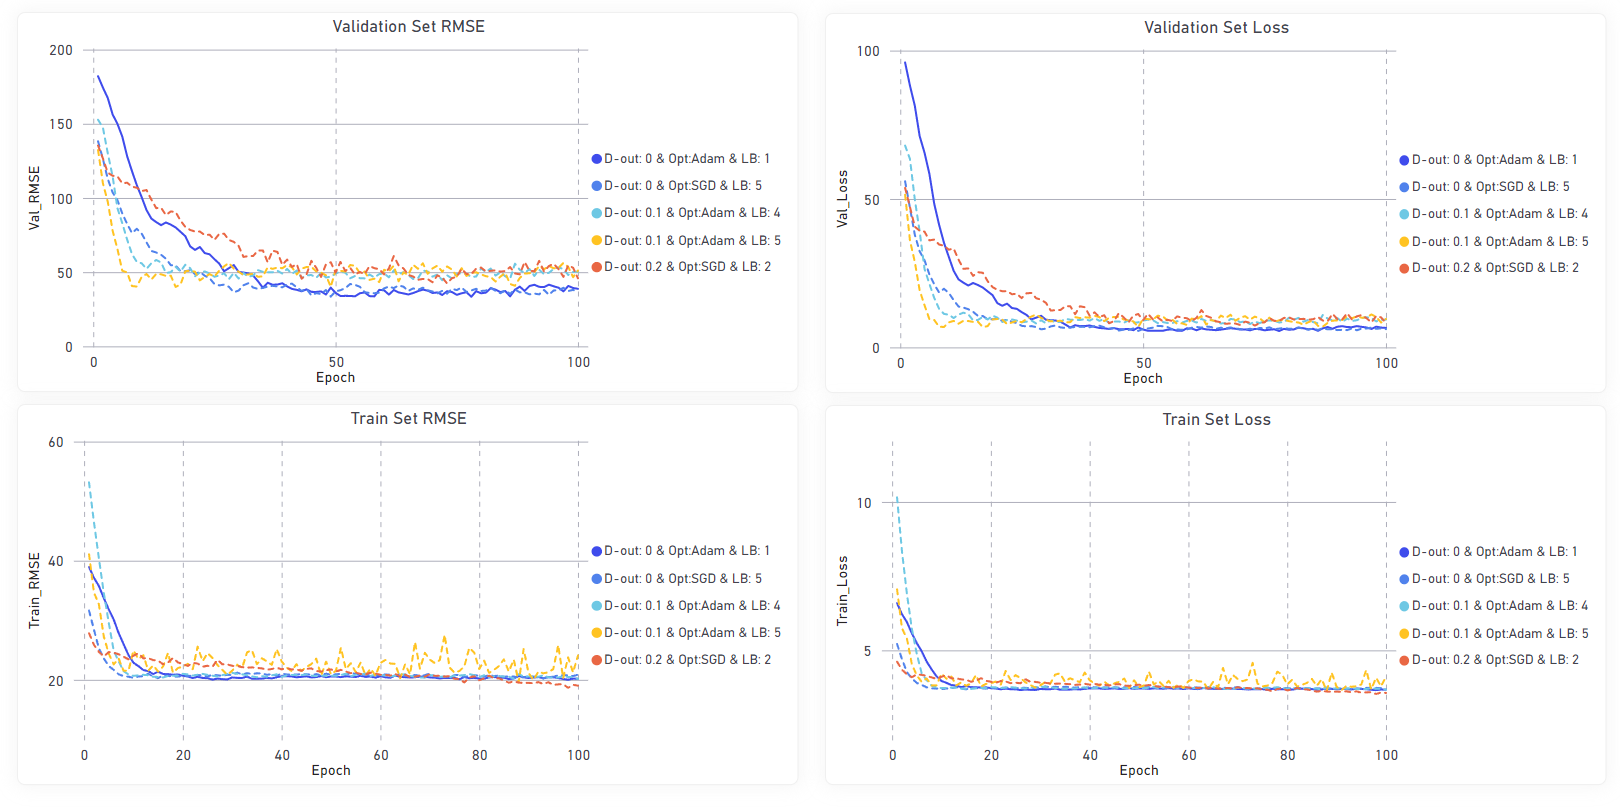
\includegraphics[width=\textwidth]{Only_Trading_Volume.png}
    \caption{5 Best Hyperparameters of LSTM Time-Series Model That Uses Price and Trading Volume}
\end{figure}

\begin{figure}
    \centering
    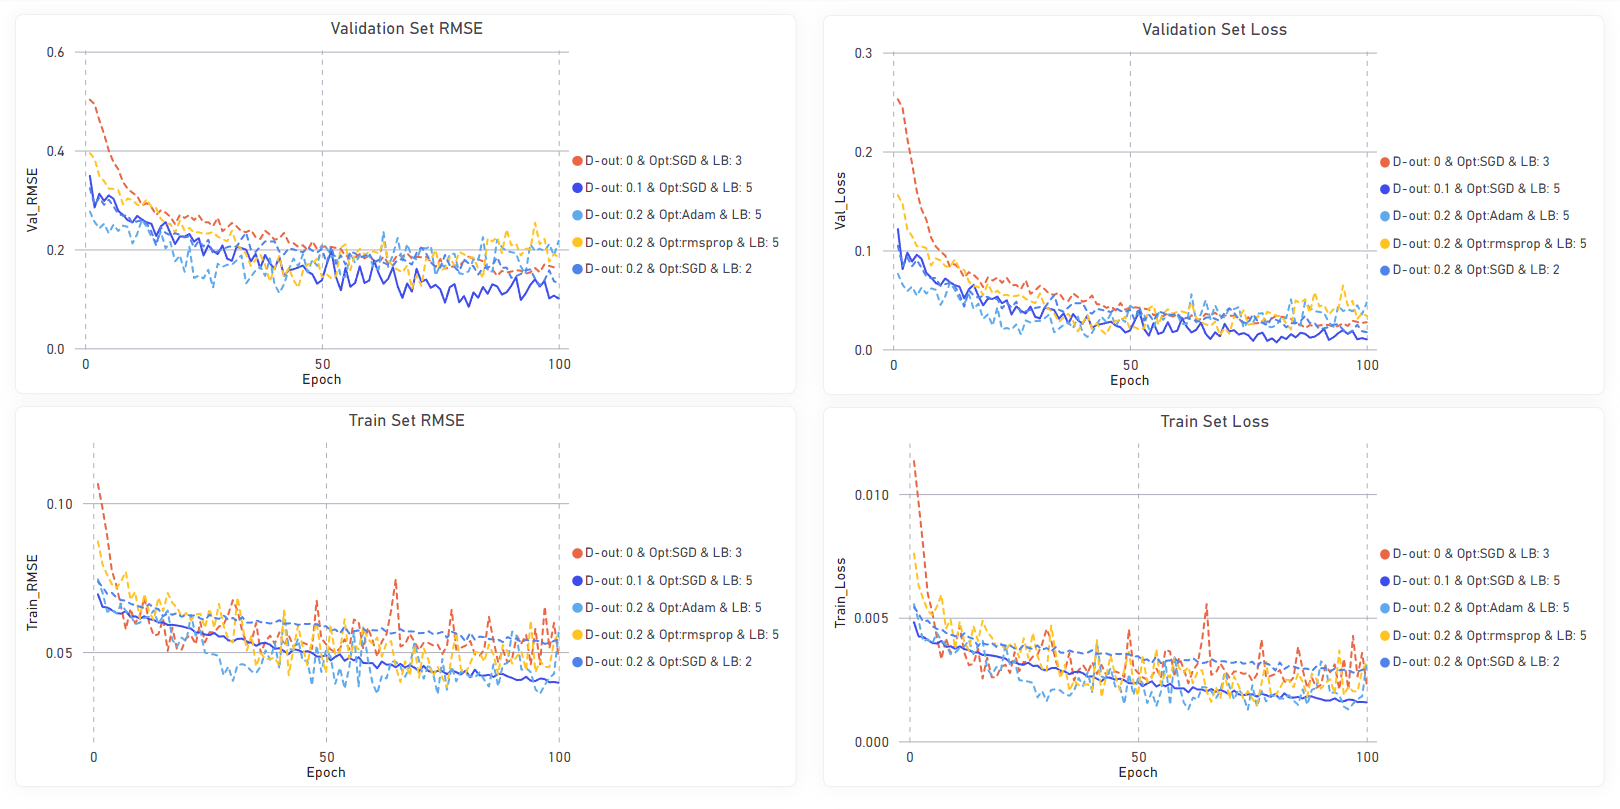
\includegraphics[width=\textwidth]{Only_Sentiment.png}
    \caption{5 Best Hyperparameters of LSTM Time-Series Model That Uses Price and Sentiment}
\end{figure}

\begin{figure}
    \centering
    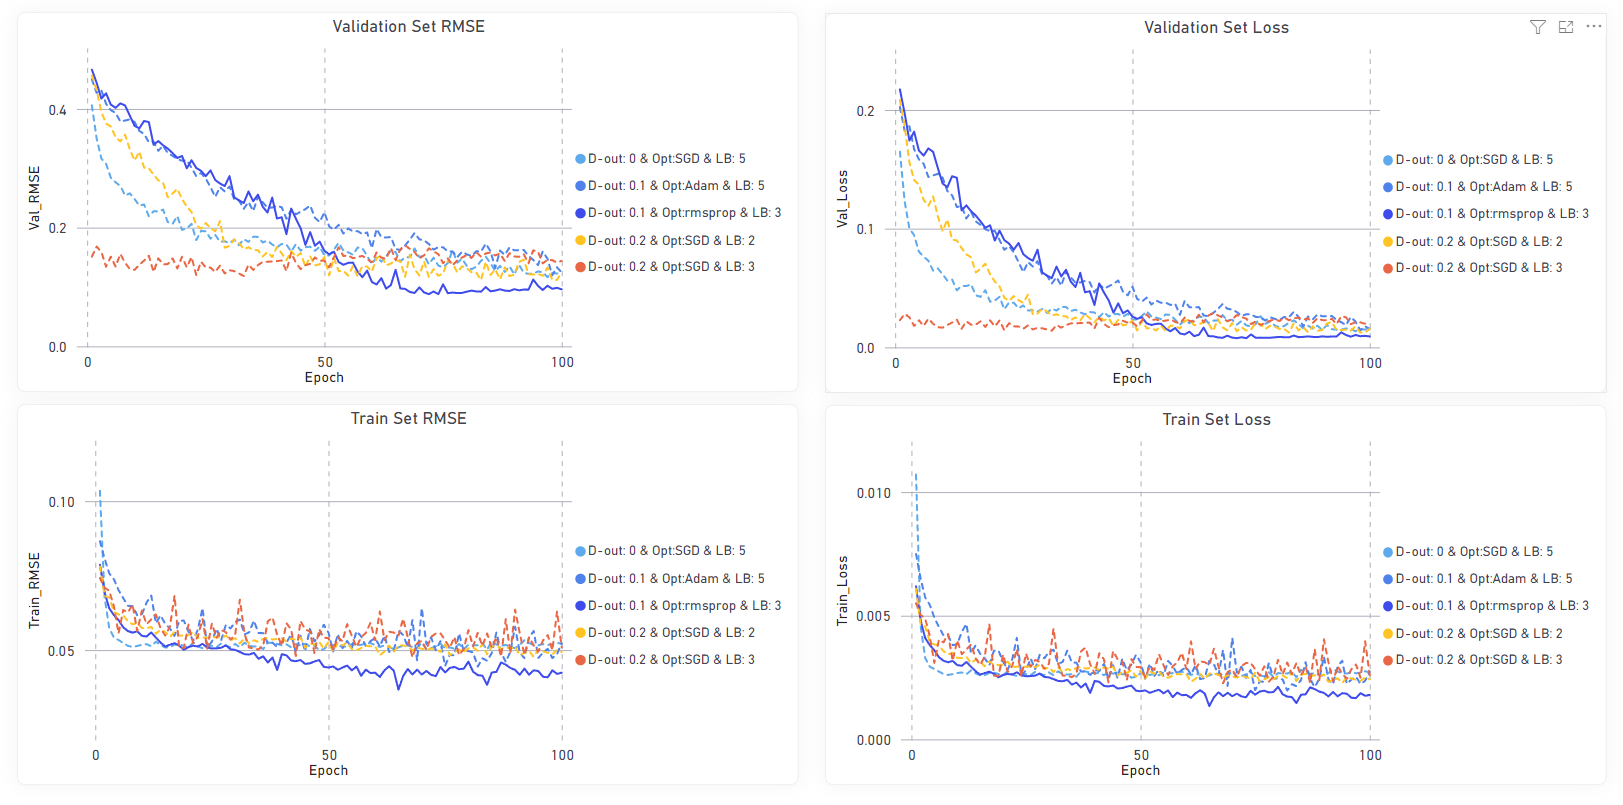
\includegraphics[width=\textwidth]{All_Features.png}
    \caption{5 Best Hyperparameters of LSTM Time-Series Model That Uses Price, Trading Volume and Sentiment}
\end{figure}

\pagebreak
\subsection{Appendix Forecast}
\label{appendix:Forecast}
As can be seen in Figure \ref{fig:arima_prediction_test_set} the ARIMA model simply seems to extrapolate the previous trend into the future.
In contrast, Figure \ref{fig:model_only_trading_volume_forecast_test_set} represents the model with the best metrics on the test set, which shows quite strong predictive results.
Based on Figure \ref{fig:high_lookback} it seems that if a model uses a lookback period of three or greater, its predictions
will be smoothed quite a lot.

\begin{figure}[!htb]
    \centering
    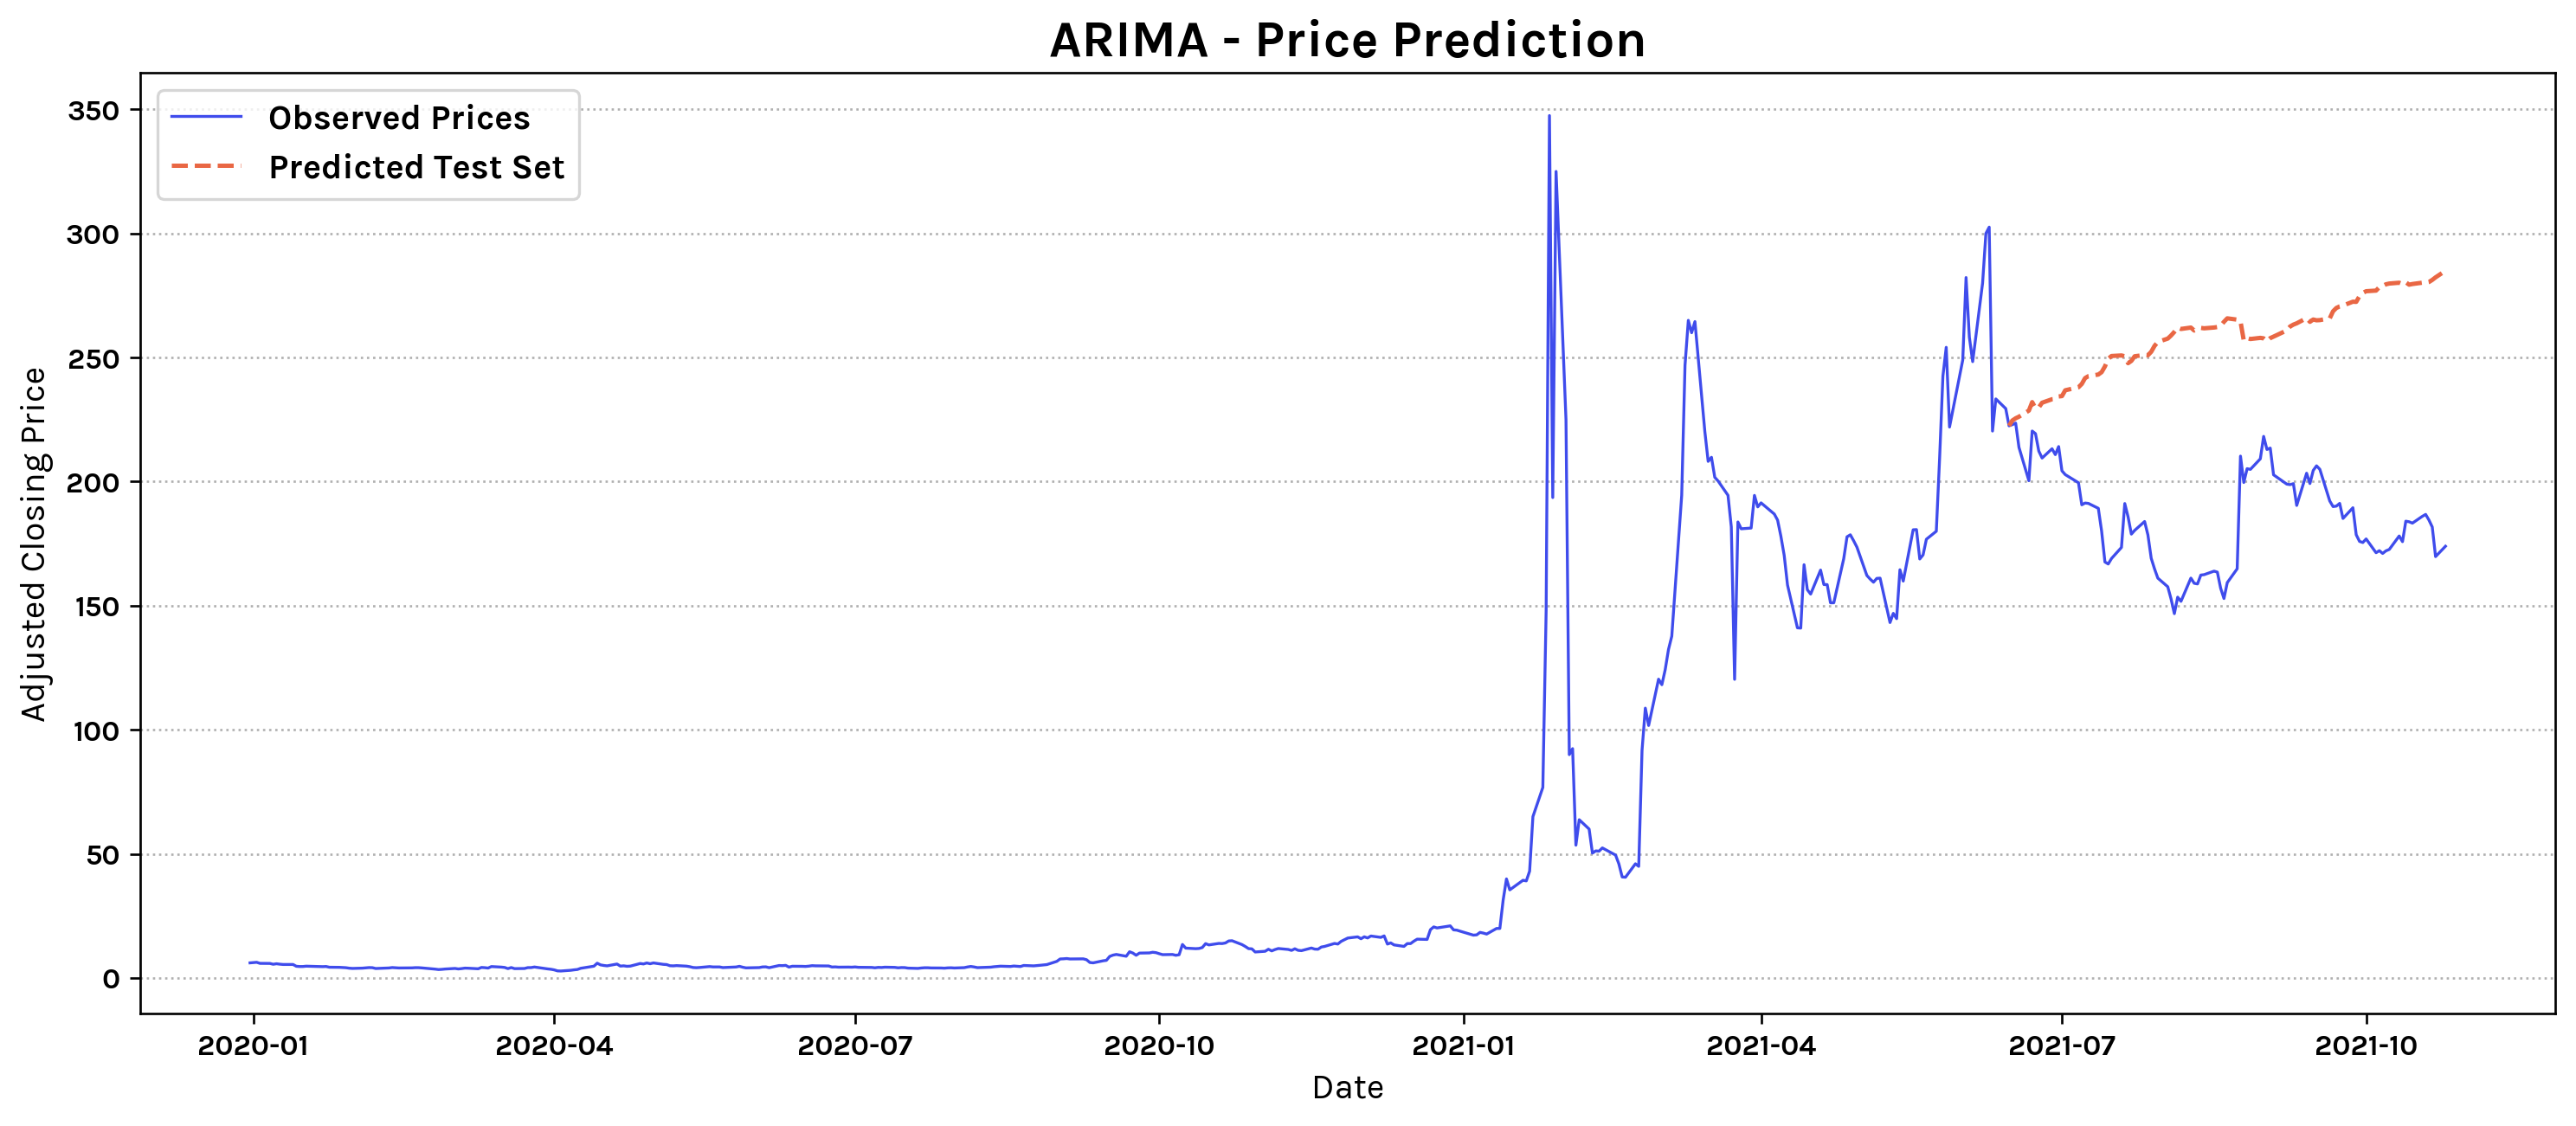
\includegraphics[width=\textwidth]{prediction_arima_pred.png}
    \caption{Forecast of ARIMA Model}
    \label{fig:arima_prediction_test_set}
\end{figure}

\begin{figure}[!htb]
    \centering
    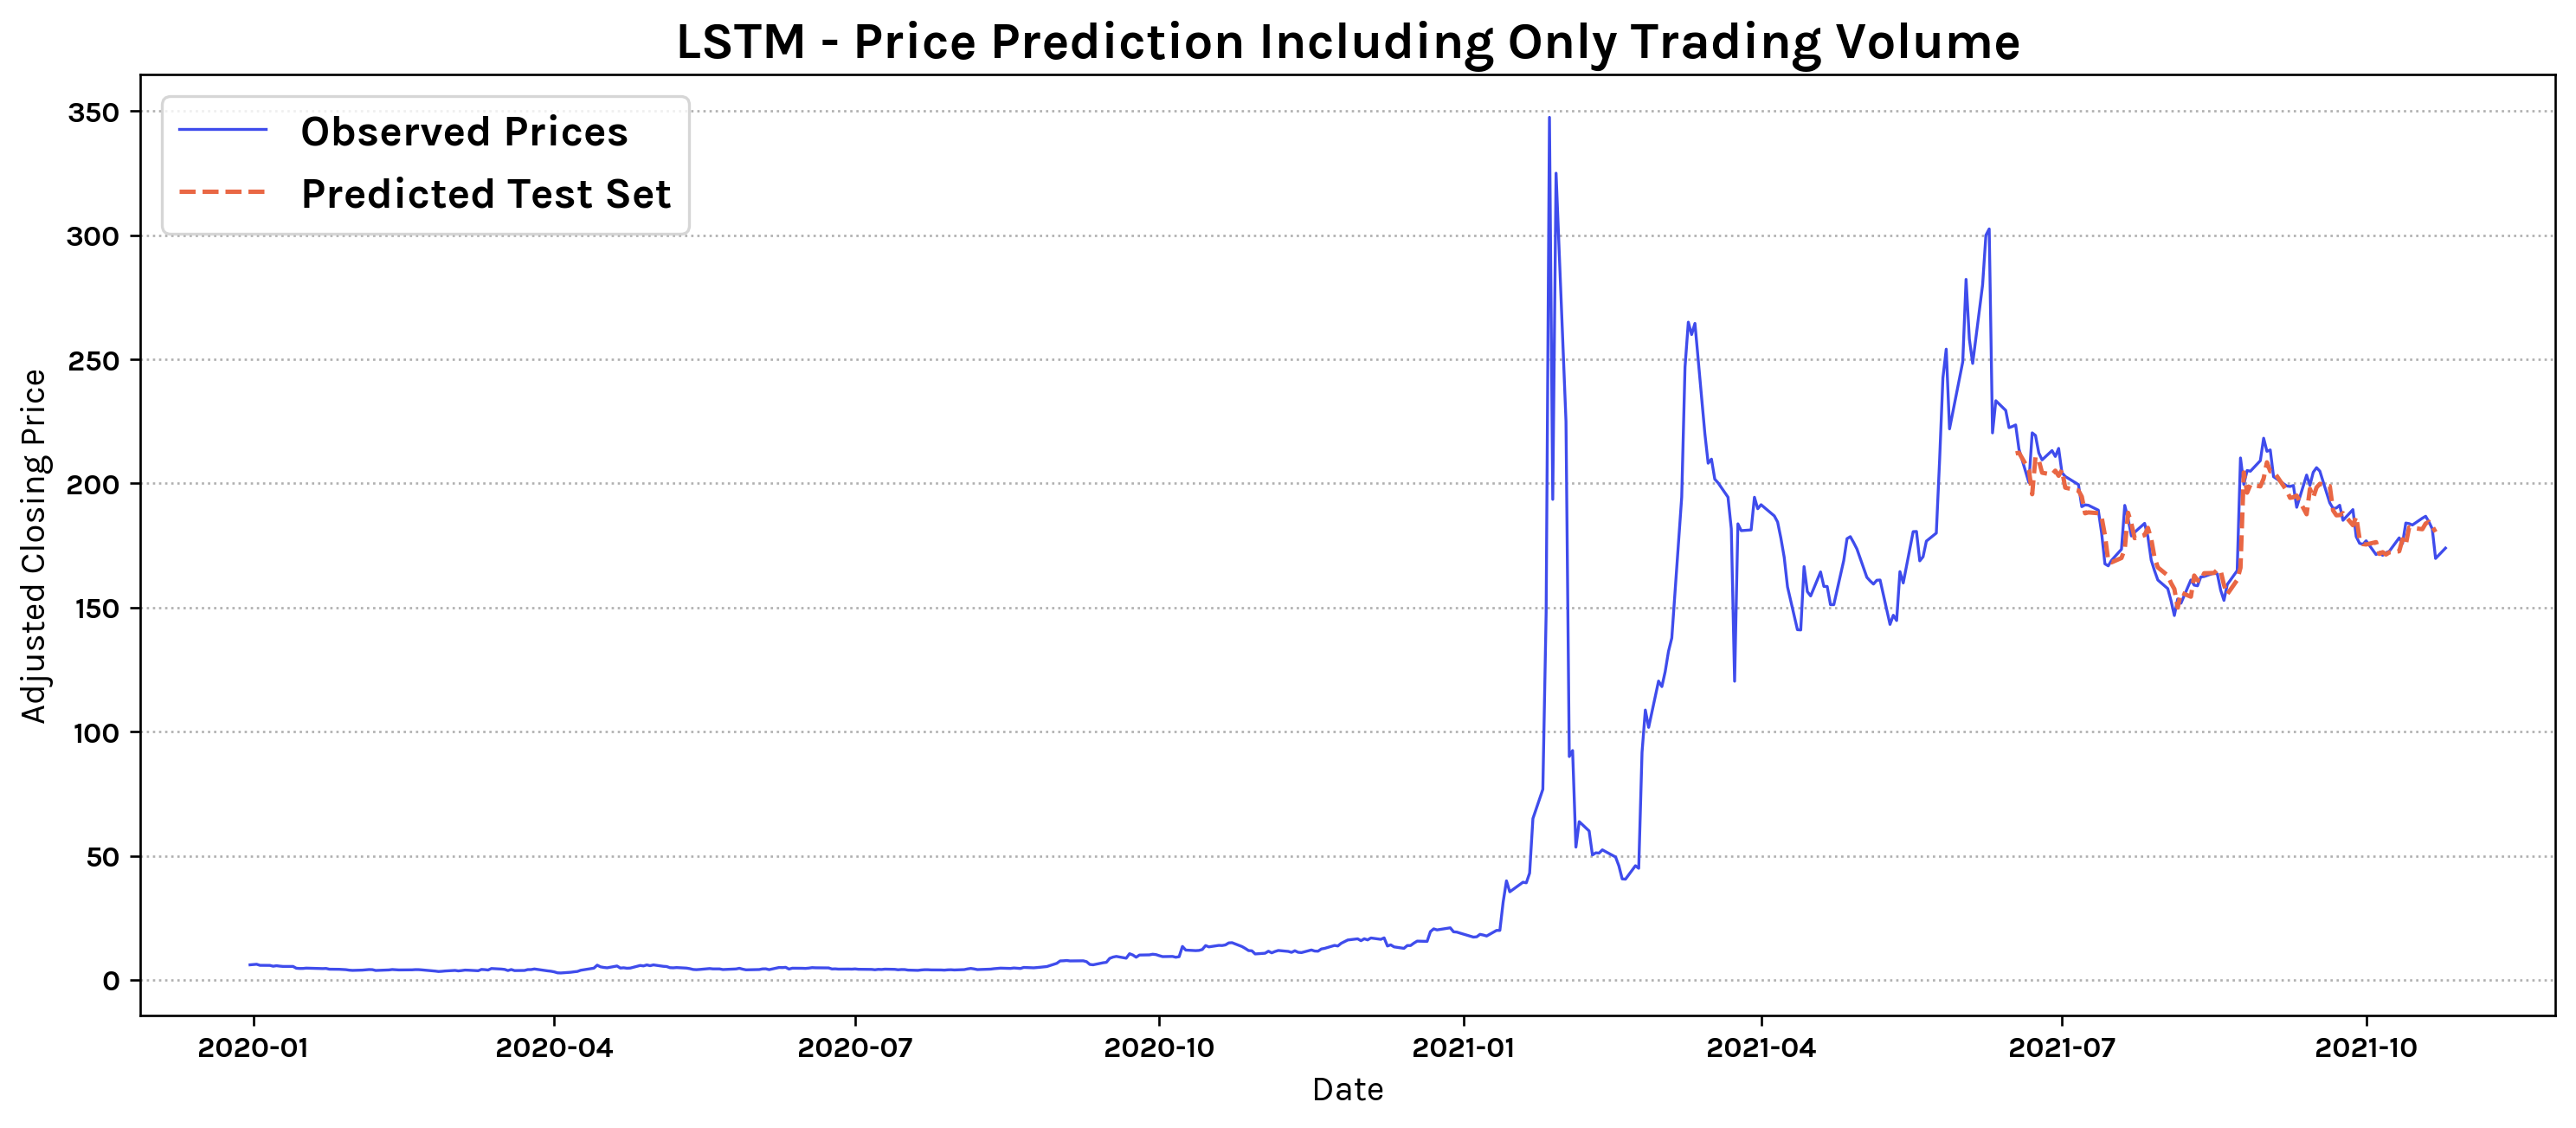
\includegraphics[width=\textwidth]{only_trading_volume_pred.png}
    \caption{Forecast of Model with Best Metrics on Test Set}
    \label{fig:model_only_trading_volume_forecast_test_set}
\end{figure}

\begin{figure}[!htb]
    \centering
    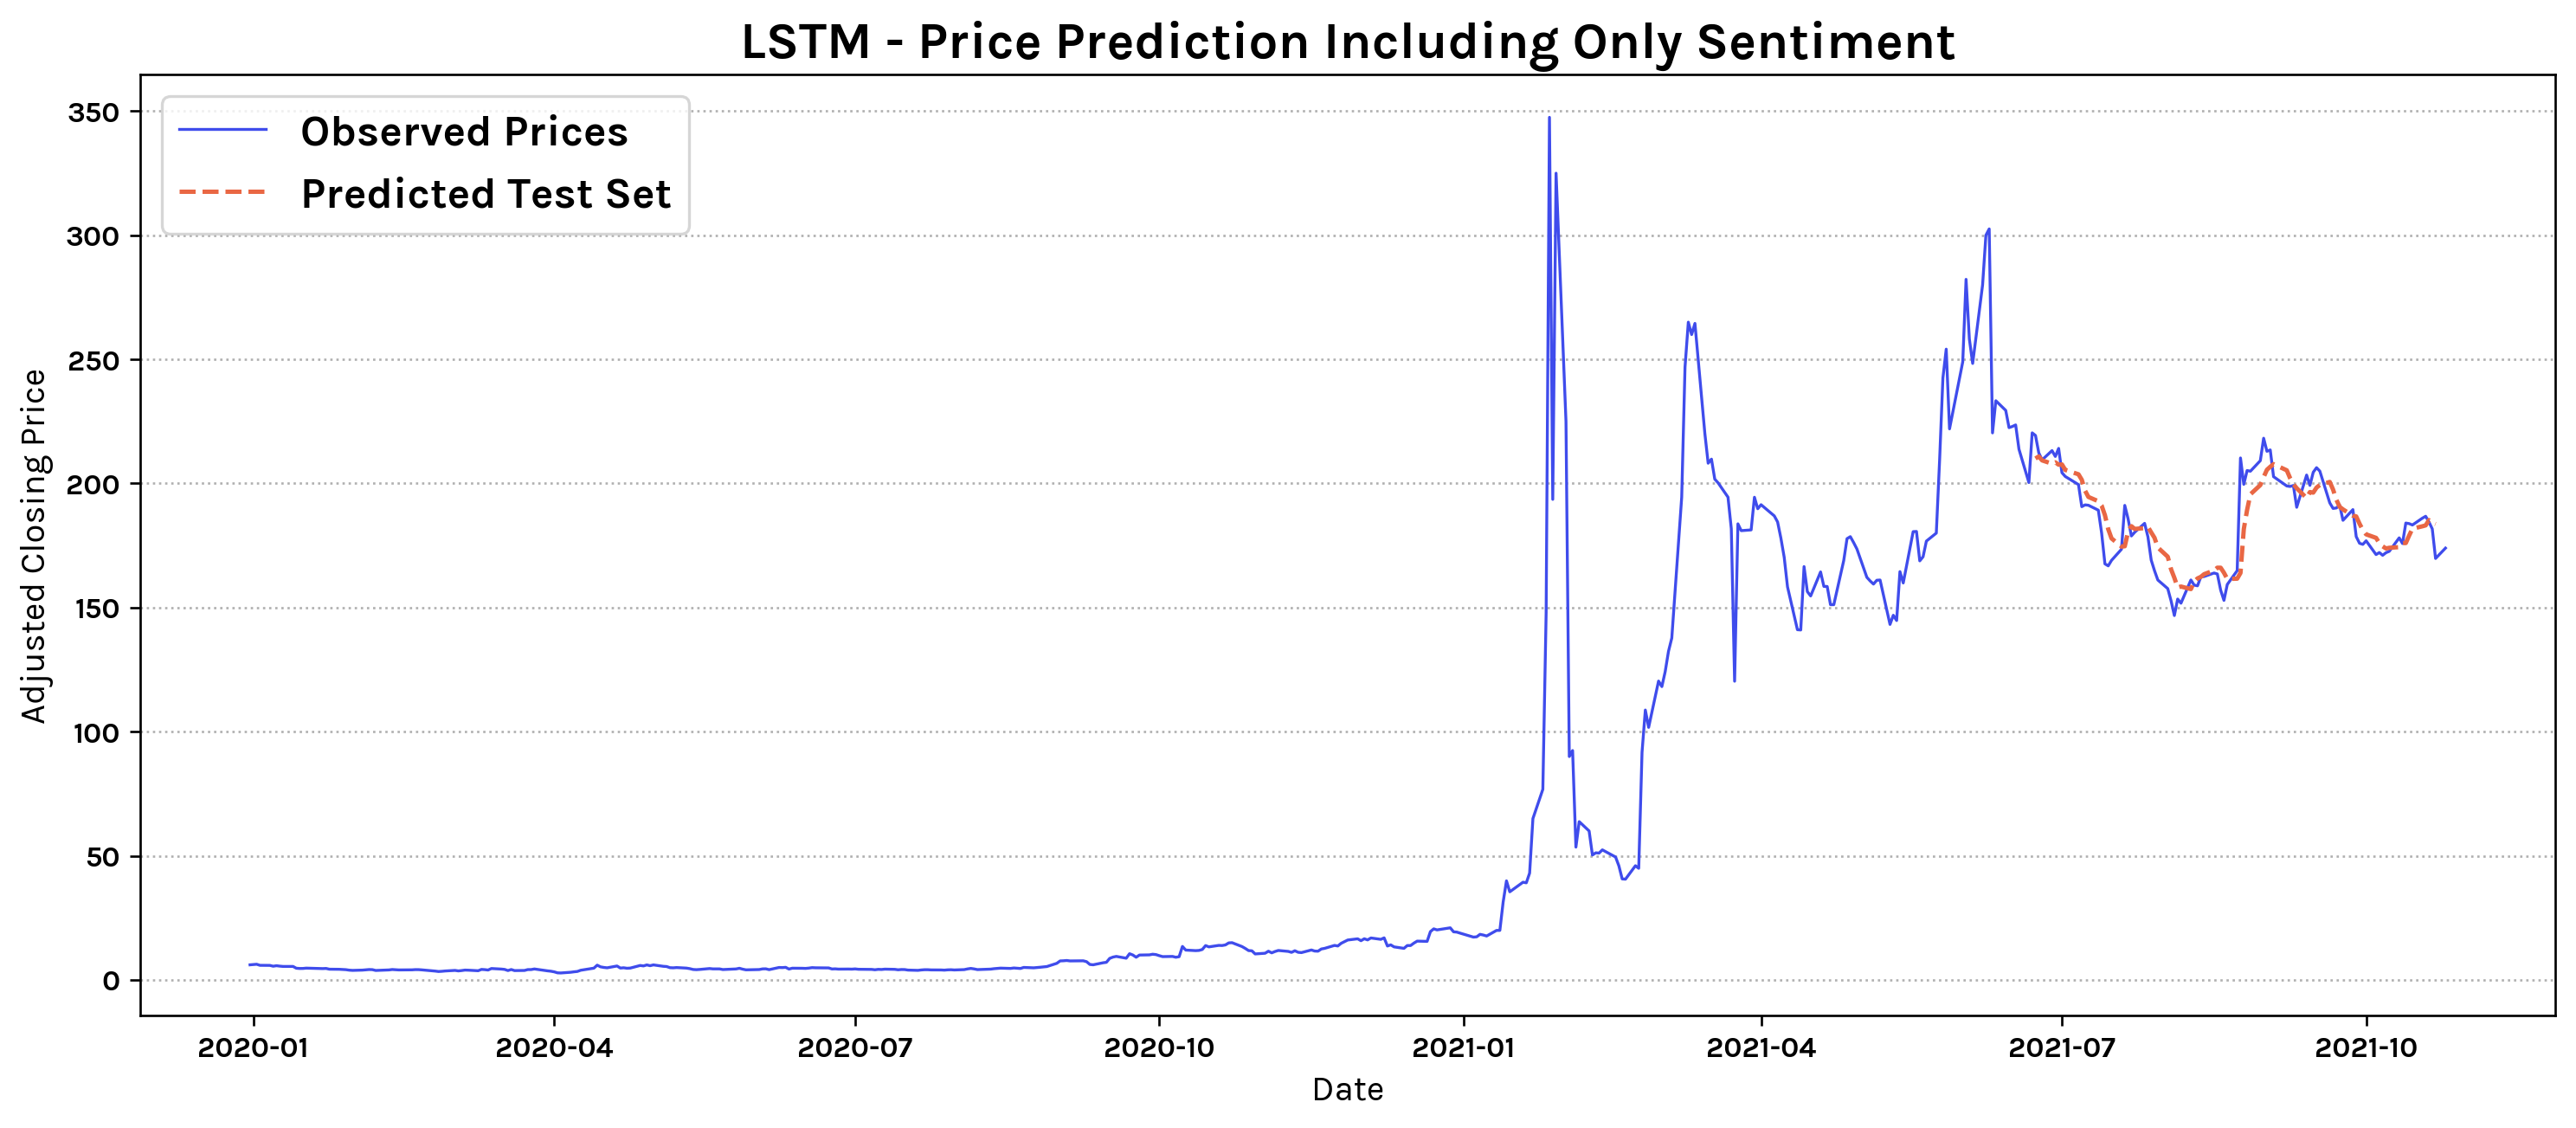
\includegraphics[width=\textwidth]{only_sentiment_pred.png}
    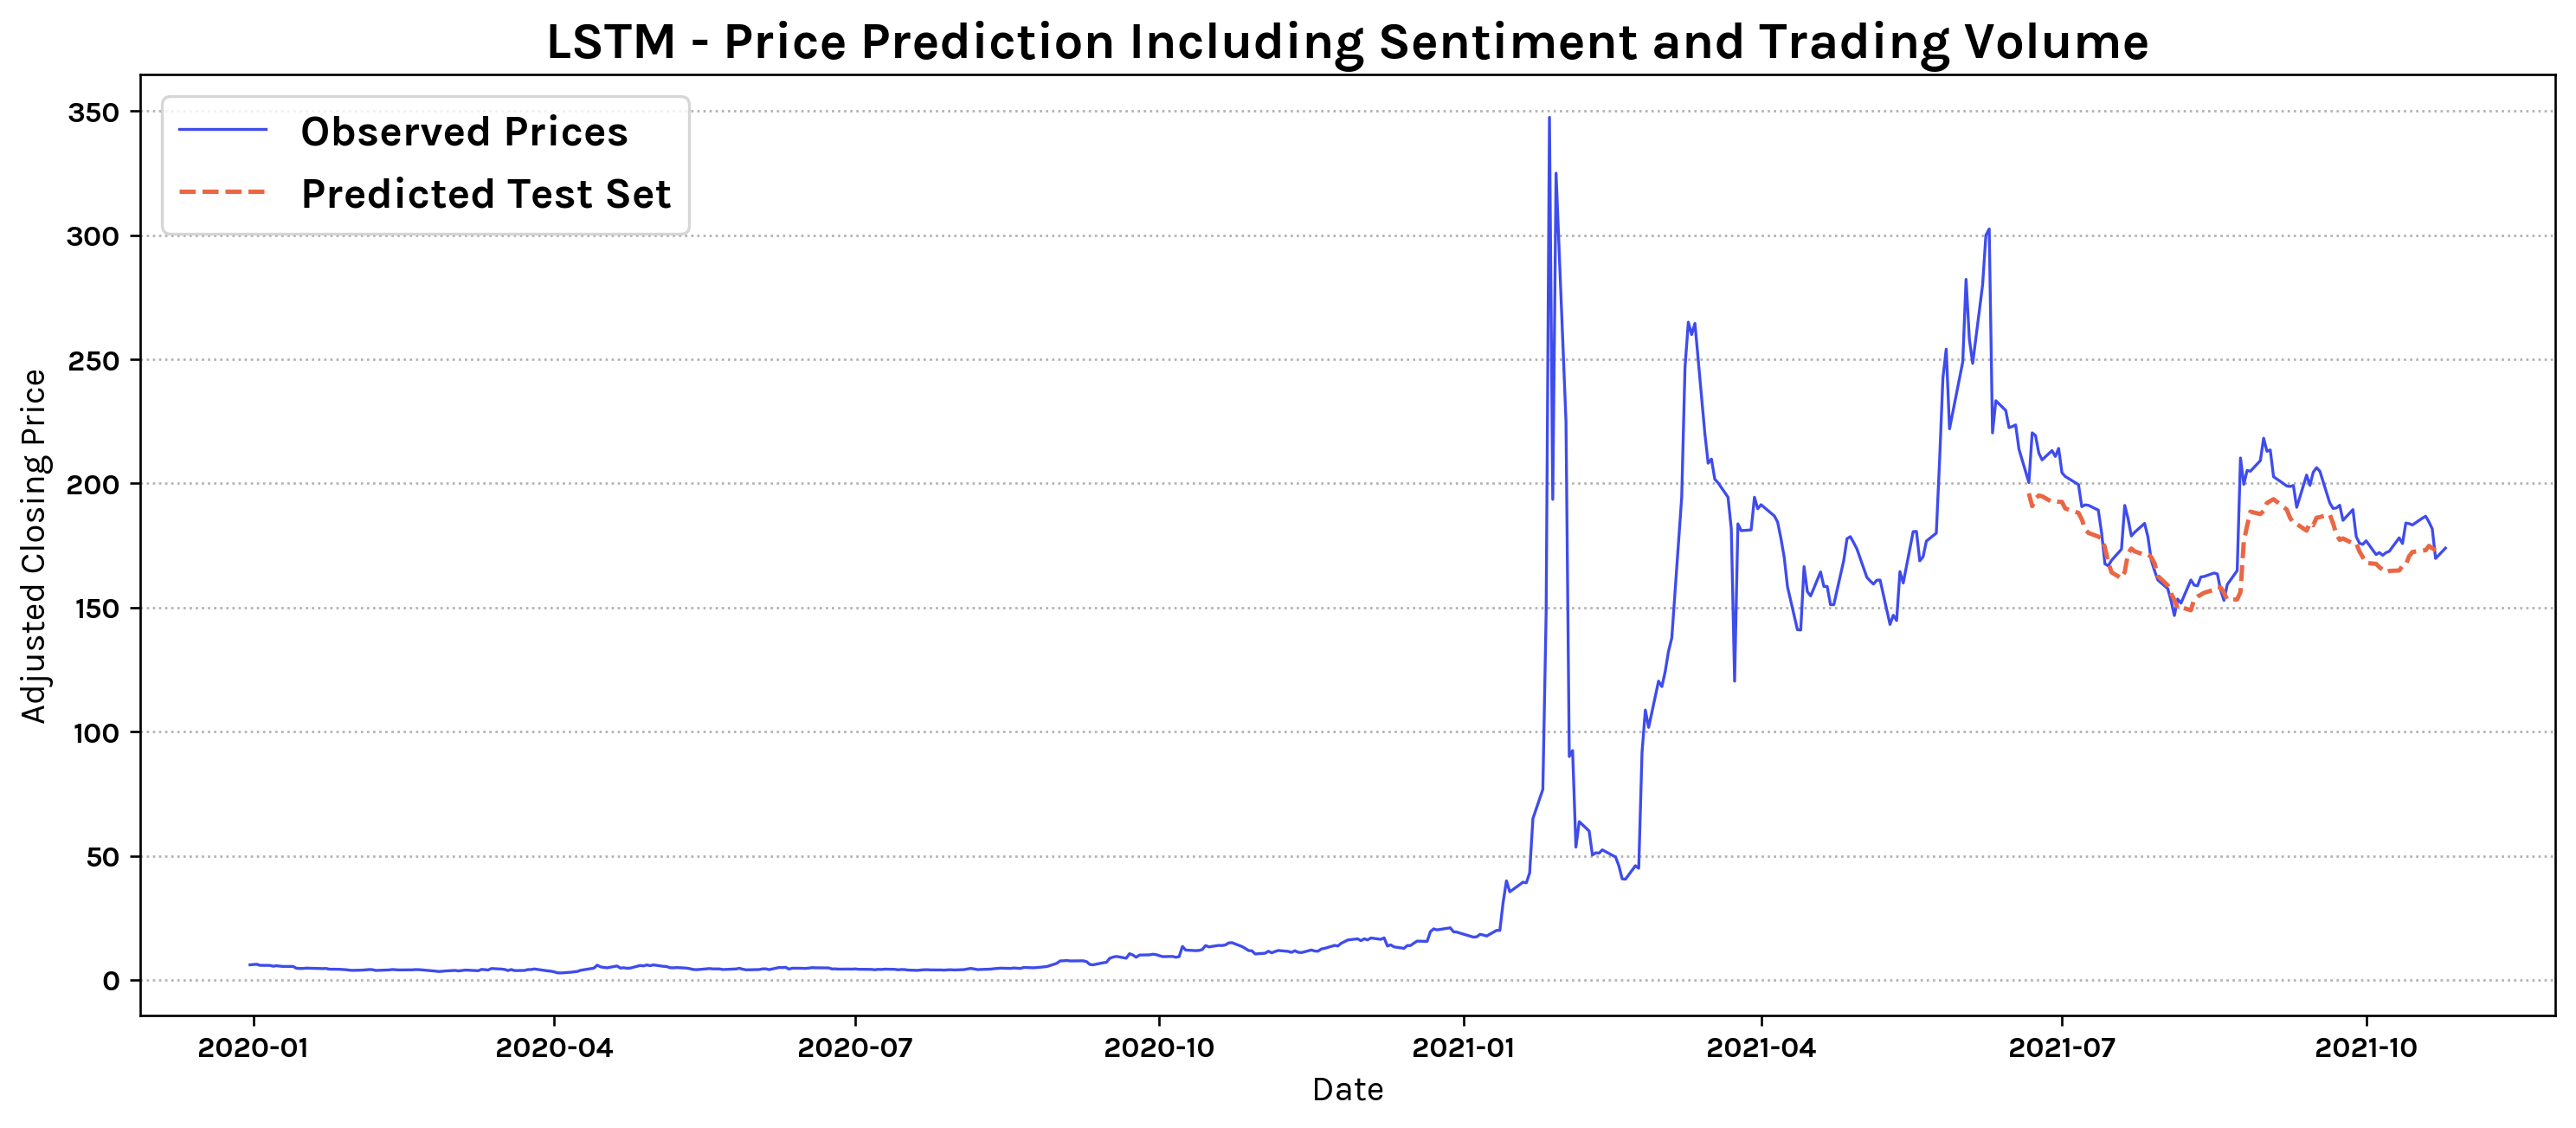
\includegraphics[width=\textwidth]{all_features_pred.png}
    \caption{Forecast of Models with Higher Lookback}
    \label{fig:high_lookback}
\end{figure}

\end{document}